\documentclass[twoside,english]{uiofysmaster}
\geometry{a4paper,includeall,bindingoffset=0cm,margin=3cm,
            marginparsep=0cm,marginparwidth=0cm,top=2cm}
\usepackage{braket}
\usepackage{mathtools}      
\usepackage{tabularx}
\usepackage{amsmath} 
\usepackage{listings}
\usepackage{color}
\usepackage{multirow}
\usepackage{lscape}
\definecolor{mygreen}{rgb}{0,0.6,0}
\definecolor{mygray}{rgb}{0.5,0.5,0.5}
\definecolor{beaublue}{rgb}{0.74, 0.83, 0.9}
\definecolor{mymauve}{rgb}{0.58,0,0.82}
\colorlet{NextBlue}{beaublue!20}
\lstset{ %
	backgroundcolor=\color{NextBlue},   % choose the background color
	basicstyle=\footnotesize,        % size of fonts used for the code
	breaklines=true,                 % automatic line breaking only at whitespace
	captionpos=b,                    % sets the caption-position to bottom
	commentstyle=\color{mygreen},    % comment style
	escapeinside={\%*}{*)},          % if you want to add LaTeX within your code
	keywordstyle=\color{blue},       % keyword style
	stringstyle=\color{mymauve},     % string literal style
	columns=flexible,
}

\usepackage{tikz}
\include {ccdiag}
\usetikzlibrary{calc,matrix}


%%%%%%%%%%%%%%%%%%%%%%%%%%%%
\usetikzlibrary{shapes,arrows}	
\usetikzlibrary{arrows,decorations.markings}
\definecolor{decisionColor}{HTML}{DEE1B2}
\definecolor{nodeColor}{HTML}{EBFAFF}
\tikzstyle{roundrect}=[rectangle, rounded corners, minimum width=3cm, minimum height=1cm, text centered, draw=black, fill=nodeColor, text width=5cm] 
\tikzstyle{roundrectSmall}=[rectangle, rounded corners, minimum width=2cm, minimum height=2cm, text centered, draw=black, fill=nodeColor, text width=3cm] 
\tikzstyle{decision} = [diamond, minimum width=3.7cm, minimum height=3.2cm, text centered, draw=black, fill=decisionColor, scale=1, text width=2.05cm]
\tikzstyle{arrow} = [decoration={markings,mark=at position 1 with
	{\arrow[scale=1.5,>=stealth]{>}}},postaction={decorate}]
%https://tex.stackexchange.com/questions/50780/arrows-at-right-angles-on-a-tikzpicture-matrix
\tikzset{
	desicion/.style={
		diamond,
		draw,
		text width=3em,
		text badly centered,
		inner sep=0pt
	},
	block/.style={
		rectangle,
		draw,
		text width=10em,
		text centered,
		rounded corners
	},
	cloud/.style={
		draw,
		ellipse,
		minimum height=2em
	},
	descr/.style={
		fill=white,
		inner sep=2.5pt
	},
	connector/.style={
		-latex
	},
	rectangle connector/.style={
		connector,
		to path={(\tikztostart) -- ++(#1,0pt) \tikztonodes |- (\tikztotarget) },
		pos=0.5
	},
	rectangle connector/.default=-2cm,
	straight connector/.style={
		connector,
		to path=--(\tikztotarget) \tikztonodes
	}
}
\usetikzlibrary{shapes,arrows}
\usepackage{tcolorbox}
\author{Anna Gribkovskaya}
\title{\uppercase{Stochastic Approach to Many-Body problems}}
\date{August 2018}
\usepackage{pdfpages}
\usepackage{mathrsfs}
\usepackage{simpler-wick}
\theoremstyle{definition}
\newtheorem{defn}{Definition}
\newtheorem{post}{Postulate}
\usepackage{bm}
\newcommand{\bmat}[2]{\begin{bmatrix}[#1] #2 \end{bmatrix}} 
\usepackage[backend=bibtex]{biblatex}
\addbibresource{master.bib} 
\pgfdeclarelayer{background}
\pgfdeclarelayer{foreground}
\pgfsetlayers{background,main,foreground}


\begin{document}

\begin{titlepage}
..\maketitle
\end{titlepage}
\begin{abstract}
	This is an abstract text.
\end{abstract}

\begin{dedication}
	To someone
	\\\vspace{12pt}
	This work is dedicated to my family. Thank you all for bearing with my while I was writing it.
\end{dedication}
\begin{acknowledgements}
	I acknowledge my acknowledgements.
\end{acknowledgements}
\tableofcontents

%\chapter{}
\chapter*{Introduction}

\section*{Motivation}
The Quantum Monte Carlo methods have been known for decades now, since in 1950  Forsythe and Leibler have presented the method for matrix inversion by stochastic approach \cite{forsytheMatrixVersionMonte1950}. However it was first applied to the physical problem in the 1962 by Kalos to compute the ground state for three- and four-body nuclei \cite{kalosMonteCarloCalculations1962}. Nowadays the Monte Carlo methods are widely used in computational physics and chemistry.\\
In this thesis we focus on an \textit{ab initio} algorithm to compute the ground state properties of a quantum system known as  Coupled Cluster Quantum Monte Carlo (CCQMC). This algorithm is based on the Full Configuration Monte Carlo (FCIQMC) developed by Booth and Alavi \cite{boothApproachingChemicalAccuracy2010} and was first introduced by Thom \cite{thomStochasticCoupledCluster2010}. We 

	
\part{Theory}
\chapter{Quantum mechanics}
In the end of 19th century physics had some unsolved problems that couldn't be tackled using already developed theories and methods. This had led to a  significantly different theory with a number of essential distinctions  from that developed before. This new theory was named quantum mechanics. In the classical (or Newtonian mechanics) there is a theoretical possibility to obtain a complete knowledge of the system under consideration. In quantum mechanics this is not possible, neither for some particular moment in time  nor for all other  moments in time. \\
Let's introduce some concepts here. The \textbf{uncertainty principle} and the \textbf{probability interpretation of the wave function}. The  uncertainty principle (or Heisenberg's uncertainty principle) puts a limit on the precision of our measurement of some particular pairs of physical quantities (e.i. position and momentum). The probability interpretation of the wave function is a bit harder to explain, because one needs a proper mathematical description of the quantum mechanics to understand this. For now we just say that if we consider one single particle in space the probability of finding it in some certain position is related to the wave function. We will derive the expression for the total wave function of the system later in this thesis. Another 
substantial difference is associated with so-called \textbf{principle of complementarity}. It was formulated by  Niels Bohr, one of the founders of the quantum mechanics. It stands that in order to describe a system we need a pair of certain complementary properties which cannot be observed simultaneously. A good example of such a pair are wave and particle properties of light or electrons. Classical mechanics considered light as a wave and electron as a particle, but this approach failed to explain the photoelectric effect and the diffraction of electrons on a slit. Moreover, position and momentum of the particle also can be considered as a pair of complementary properties. This makes Bohr's principle of the complementarity closely connected to Heisenberg's uncertainty principle. Also one should mention that quantum mechanics allows us to change the number of particles in some particular state. For example, we have a \textbf{creation} operator which increases the number of particles in some given state of the system by one, and \textbf{annihilation} operator which decreases this number by one. The last concept to be mentioned here is the word \textbf{quantum} itself. In physics, "quantum" determines the smallest possible difference between two values or minimal amount of quantity involved in an interaction. This concept is associated with the revolutionary supposition made by Max Planck back in 1900. He assumed that electromagnetic energy could be emitted in a form of some discrete quantities, known as “quantum”. He also introduced a proportionality coefficient for a minimal energy difference, so-called Planck's constant $h = 6.626 \times 10^{-34} \text{ } (kg \cdot m^2\cdot s^{-1})$. As one can see it has a very small value.  \\
How does it possible to have two theories much different from each other and continue to use both of them? This is perfectly fine even it may seems to be a bit contradictory. In science there is a rule that require for any new theory to agree with the previous ones under some conditions. This rule is called a \textbf{correspondence principle}. In case of quantum mechanics these conditions are named \textbf{classical limit} or \textbf{correspondence limit}. In particular this means that quantum mechanical description of the system should correspond to those obtained by classical theory for large quantum numbers. Mathematically it can be achieved by requirement $h \rightarrow 0$, where $h$ Planck's constant. This principle allows us to determine whether a specific quantum theory is valid or not.\\
Today we usually say that classical mechanics describes the macroscopic objects and quantum mechanics describes microscopic ones. This arise from the fact that some quantum effects can be observed only for extremely small particles. However this is not enough to describe the difference, because even the observation itself is now different from that in classical physics. 
For more details on the matter, please refer to \cite{phillipsIntroductionQuantumMechanics2003}. \\


\section{Quantum theory}
In this section we provide a brief description of main assumptions needed for the quantum theory and  some basic notations to be used in the thesis.\\
As it has been already mentioned quantum theory has been developed though the $20^{\text{th}}$ century. As any other new theory it is based on some assumptions called the postulates of quantum mechanics (QM). In this thesis we do not aim to provide a detailed description on the topic, however some basic introduction is needed.\\

\begin{defn} Hilbert Space.\\
	Let $\mathscr{H}$ be a complex vector space. The inner product $\braket{\alpha|\beta} $\footnote{$\ket{\alpha}$ and  $\ket{\beta}$ are ket-vectors in Dirac notations.} in that space is defined so that it has the following properties:
	\begin{enumerate}		
		\item $\braket{a\alpha|\beta} = a\braket{\alpha|\beta}$, $a \in C$.
		\item $\braket{\alpha|b\beta} = b^{*}\braket{\alpha|\beta}$, $b \in C$.
		\item $\overline{\braket{\alpha|\beta}} =\braket{\beta|\alpha}$.
		\item $||\alpha||^2= \braket{\alpha|\alpha} \geq 0 $.			
	\end{enumerate}
\end{defn}

\begin{post}
	Every instant state of a system is represented by a vector in Hilbert space $\mathscr{H}$.\\
\textit{Comment}. This is a very strong demand, because it means that any superposition of the different states is also a state of the system. For example, if $\ket{\alpha_1}$ and  $\ket{\alpha_2}$ are vectors describing possible states of the system, then their linear combination $\ket{\alpha}$ is also a state of the same system:
\begin{equation*}
\ket{\alpha}=a_1\ket{\alpha_1}+a_2\ket{\alpha_2}, \text{   } a_1\text{  and }  a_2 \in C.
\end{equation*}
\end{post}
\begin{defn}
Operator $\hat{Q}$ is Hermitian if it satisfies the equation:
\begin{equation}
\hat{Q}^\dagger=\hat{Q},
\end{equation}
where $\hat{Q}^\dagger$ is adjoint of $\hat{Q}$.
\end{defn}
\begin{post}\label{postulat2}
	Every physical observable is associated with an operator $\hat{Q}$ in a Hilbert space. Action of the operator on state vector results into following eigenvalue equation:
	\begin{equation}\label{eq:general_eigval eq}
	\hat{Q}\ket{\alpha}= q\ket{\alpha}, 
	\end{equation}
where eigenvalues $q$ are the only measurable values associated with the operator. Eigenvectors determine a complete orthonormal set of vectors for this operator. In addition every operator $\hat{Q}$ associated with a measurable physical quantity must be a linear Hermitian operator. In particular that means it should posses the following properties:
	\begin{align}
	&\hat{Q}^\dagger=\hat{Q},\\
	&(a\hat{Q})^\dagger=a^*\hat{Q}^\dagger,\\
	&(\hat{Q}\hat{P})^\dagger  =\hat{P}^\dagger \hat{Q}^\dagger,\\
	&(\hat{Q}+\hat{P})^\dagger =\hat{Q}^\dagger+\hat{P}^\dagger,
	\end{align}
	where $a \in C$, and * denote complex conjugate.\\
\textit{Comment}. The eigenvalue equation ($\ref{eq:general_eigval eq}$) has interesting properties when $\hat{Q}$ is Hermitian operator. They are presented in theorems below.
\end{post}

\begin{theorem}\label{theorem:eigvalHerm}
	Set of eigenvalues of any Hermitian operator $\hat{Q}$ on Hilbert space $\mathscr{H}$ is set of real numbers. 
\end{theorem}

\begin{theorem}\label{theorem:eigvecHerm}
	Eigenvectors of any Hermitian operator $\hat{Q}$ on Hilbert space $\mathscr{H}$ that belong to different eigenvalues are orthogonal. 
\end{theorem}

\begin{theorem}\label{theorem:orhtonormalbasis}
Set of eigenvectors of any Hermitian operator $\hat{Q}$ on Hilbert space $\mathscr{H}$ can be chosen to be an orthonormal basis for $\mathscr{H}$.
\end{theorem}
We do not provide proofs for these Theorems. For more detailed description please refer to \cite{aulettaQuantumMechanics2009}.
\begin{post}
	Let $\mathscr{H}_1$ and $\mathscr{H}_2$ be the Hilbert spaces corresponding to two systems. The Hilbert space of joint system is given by tensor product $\mathscr{H}=\mathscr{H}_1 \otimes \mathscr{H}_2$.\\
\textit{Comment}. As it is shown further in this thesis this postulate provides a method to describe many-particle systems. 
\end{post}
\begin{post}
The time evolution of the quantum mechanical system is given by the Schr\"{o}dinger equation:
\begin{equation}\label{eq:basic_schrod}
 i \hbar \frac{\partial }{ \partial t}\ket{\Psi} = \hat{H}\ket{\Psi},
\end{equation}
where $\ket{\Psi}=\ket{\Psi(t)}$ .
\end{post}
In this thesis we do not consider time-evolution of the system and will be focused on the time-independent Schr\"{o}dinger equation or stationary-state equation:
\begin{equation}
\hat{H}\ket{\Psi} = E \ket{\Psi},
\end{equation}
where $\hat{H}$ in Hamiltonian, $\ket{\Psi}$ is state vector of the system and $E$ is the expectation value of the energy. It is the energy spectrum we are interested in, so before solving the Schr\"{o}dinger equation we need to agree on the form of Hamiltonian and also construct the state vector. This is presented in the sections below.


\subsection{Many-Body problem formulation}

As it has been already mentioned all state functions arethe  vectors in the Hilbert space. When we deal with a system consisting of many particles we need to define the type of these particles. Bosons are the particles with an integer spin and fermions are the particles with an odd half-integer spin. State vectors of these particles belong to different Hilbert spaces and should be studied independently. In this thesis we consider electrons which are fermions and must obey an exclusion principle, formulated by Wolfgang Pauli in 1925.
\begin{defn}The Pauli exclusion principle.\\
Two or more identical fermions cannot occupy the same quantum state simultaneously in the same system.
\end{defn}
Let's take a closer look at the total wave function and how this principle affect the permutations of the particles withing the system. First we need to mention that the particles are identical and indistinguishable. In quantum mechanics interacting and identical particles are considered indistinguishable, which is different from classical mechanics where all particles are distinguishable. The concept of indistinguishability requires some discussion about what happens to the wave function if we interchange the particles? At this point a difference between bosons and fermions becomes a significant issue. \\
In order to make a proper mathematical description and be able to drive properties of wave functions we need to define a new operator for permutation of the particles.\\
\begin{defn}\label{denf:permutation}
Let $\hat{P_{ij}}$ be the operator that interchanges particles $i$ and $j$. 
\[\hat{P_{ij}} \ket{ \Psi(x_1 ... x_i ... x_j ...) }=\ket{ \Psi(x_1 ... x_j ... x_i ...) } \]
\end{defn}
\begin{theorem} Hermiticity of the permutation operator.\\
	$\hat{P_{ij}}$ is a Hermitian operator in Hilbert space for identical particles.\\
	So that $\hat{P_{ij}}^{-1}=\hat{P_{ij}}^\dagger$.
\end{theorem}
Considering this property one may define and solve the eigenvalue equation for the permutation operator.
\begin{eqnarray}
\hat{P_{ij}}\ket{\Psi}=\epsilon_{ij}\ket{\Psi},\\
\hat{P_{ij}}\hat{P_{ij}}\ket{\Psi}= \epsilon_{ij}^2 \ket{\Psi},\\
\epsilon_{ij}^2 =1 \rightarrow \epsilon_{ij} = \pm 1.
\end{eqnarray}
\begin{defn}Symmetricity of wave function.\\
If $\epsilon_{ij}=1$,  $\ket{\Psi}$ considered to be symmetric. In this case it corresponds to bosons.\\
If $\epsilon_{ij}=-1$,  $\ket{\Psi}$ considered to be antisymmetric. In this case it corresponds to fermions.
\end{defn}
The permutation operator is used in Chapter $\ref{ch:HF}$ for construction of total many fermion wave function and in Chapter $\ref{ch:coupled_cluster}$ for amplitudes.
\subsubsection{The Hamiltonian of many-body system} \label{sec:manybody}
As it has been already mentioned Hamiltonian is a Hermitian operator. It can be expressed as follows:
\begin{equation}
\hat{H}=\hat{T}+\hat{V},
\end{equation}
where $\hat{T}$ is the kinetic energy operator and $\hat{V}$ is the potential energy operator. \\
Here we assume the electrons are confined by a pure isotropic harmonic oscillator (H.O.) potential. Also in this thesis we consider closed shell systems. It means that all possible single-particle states below a certain level are occupied. Such level often called a Fermi level of the system. In particular this assumption means that addition or removal of one electron to such system requires more energy than same the action in a system with non-occupied lowest levels. 
%That leads to a given number of particles $N = \{2, 6, 12, 20\}$ we may have in our quantum dot. 
Using natural units ($\hbar=c=e=m_e=1$) one can write Hamiltonian of a such system in Cartesian coordinates as
\begin{equation}
\label{eq:finalH}
\hat{H}=\sum_{i=1}^{N} \left(  -\frac{1}{2} \nabla_i^2 + \frac{1}{2} \omega^2r_i^2  \right)+\sum_{i<j}^{N}\frac{1}{r_{ij}},
\end{equation}
$N$ here is number of electrons, $\omega$ is oscillator frequency and $r_{ij}$ distance between two electrons. The first sum here corresponds to the harmonic oscillator and second sum corresponds to the interaction part. The Hamiltonian can be rewritten as
\begin{equation}
\hat{H}=\hat{H}_0+\hat{H}_I .
\end{equation}
%here $\hat{H}_0$ is a standard H.O. part and $\hat{H}_I$ gives a repulsive interaction part. 
%For the Hartree-Fock method we need a single-particle basis, which in this case is just a H.O. functions. However we also need to compute elements for the Coulomb interaction matrix. The details are discussed below in a method description part. 
More detailed the Hamiltonian can be written as 
\begin{equation}
\hat{H} = \sum_{i=1}^{N}\hat{h}_0(i) + \sum_{i < j}^{N}\hat{w}(i,j),
\label{H1H2}
\end{equation}
here $ \hat{h}_0(i) $ represents the kinetic energy of the particle, possibly an external potential and the $\hat{w}(i,j)$ term represents the potential energy of Coulomb interaction between two particles. 

\subsection{Second quantization}
The second quantization is a framework that allows us to write long and cumbersome expressions, such as Slater Determinants and many-body Hamiltonian, in a compact way. This is achived by the usage of so-called creation and annihilation operators.
\cite{umrigarObservationsVariationalProjector2015}
\begin{defn} Creation operator. \\
	We define creation operator as follows:
	\begin{equation}
	c_i^\dagger\ket{-}=\ket{i},
	\end{equation}
	where $\ket{-}$ is a true vacuum state.\\
	Creation operator acting on an arbitrary state of some system results into the following expression:
	\begin{equation}
	c_i^\dagger\ket{p_1 p_2  \dots p_N}=\ket{i p_1p_2 \dots p_N}	
	\end{equation}
\end{defn}
\begin{defn}
	Annihilation operator is defined as hermitian adjoint to creation operator. \\
		\begin{equation}
		c_i\ket{i}=\ket{-}	
		\end{equation}
\end{defn}
Some important results following from the definition of the operators:
\begin{enumerate}
\item $c_i \ket{-}=0$ (no particles).
\item $c_i^\dagger\ket{p_1 p_2  \dots p_N}=0$ if $i=p_i$ (particle already exists in state vector).
\item $c_i\ket{p_1 p_2  \dots p_N}=0$ if $i\neq p_i$ (particle does not exist in state vector).
\end{enumerate}
\section{Operator representation in second quantized form} \label{sec:operator in 2q}
The Hamiltonian now considered in form ($\ref{H1H2}$). Omitting the summations and presenting operators in more generic way, it can be written as:
\begin{equation}
\hat{H}=\hat{H}_0+\hat{W}
\end{equation}
where $\hat{H}_0$ is the so-called one-body term and $\hat{W}$ is the two-body term.
In a second quantized form the one-body term can be written as:
\begin{equation}
\hat{H}_0 = \sum_i^N\hat{h}(i)=\sum_{pq}^{N}\bra{p}\hat{h}\ket{q}c_p^\dagger c_q=\sum_{pq}h_{pq}c_p^\dagger c_q, \\ \label{eq:H0}
\end{equation}
where
\begin{equation}
h_{pq}=\int_{-\infty}^{\infty}\phi_p(x)^* \hat{h}\phi_q(x) dx.\\
\end{equation}
Similarly, the two-body term can be expressed as follows:
\begin{equation}
\hat{W}=\sum_{i<j}^{N} \hat{w}(i,j)=\frac{1}{2}\sum_{pqrs}^{N} w_{rs}^{pq}c_p^\dagger c_q^\dagger c_sc_r\\ \label{eq:W},
\end{equation}
where
\begin{equation}
w_{rs}^{pq}=\bra{pq}\hat{w}\ket{rs}=\int dx_1 \int dx_2 \phi_p(x_1)^*\phi_p(x_2)^* \hat{h}\phi_r(x_1)\phi_s(x_2). 
\end{equation}
As soon as we study fermions it's more convenient to write the two-body term in an antisymmetric form:
\begin{gather}\label{eq:two-body_2q}
	\hat{W}=\frac{1}{4}\sum_{pqrs} \bra{pq}\hat{w}\ket{rs}_{AS} c_p^\dagger c_q^\dagger c_sc_r,
\end{gather}
where
\begin{gather}
	\bra{pq}\hat{w}\ket{rs}_{AS}\equiv \bra{pq}\hat{w}\ket{rs}-\bra{pq}\hat{w}\ket{sr}
\end{gather}
From here on we just use antisymmetric form, so subscript \textit{AS} can be omitted.\\
The Hamiltonian in second quantized form can be then written as:
\begin{equation}\label{eq:Ham in 2q}
\hat{H}=\sum_{pq}^{N}\bra{p}\hat{h}\ket{q}c_p^\dagger c_q + \frac{1}{4}\sum_{pqrs} \bra{pq}\hat{w}\ket{rs}_{AS} c_p^\dagger c_q^\dagger c_sc_r
\end{equation}
\section{Normal ordering and Wick's theorem} \label{sec:Wick}
As it has been already mention we need second quantization to write long expressions in a compact way. However, we also need rules to deal with this expression written in a second quantized form to compute for example matrix elements of Hamiltonain matrix. After writing the Hamiltonian in a second quantized form we are able use for this purpose the following anti-commutator relations:
\begin{gather}
\{c_p,c_q \}=0\\
\{c_p^\dagger,c_q^\dagger \}=0\\
\{c_p,c_q^\dagger\} = \delta_{pq} \label{eq:fund_anti}
\end{gather}
Equation (\ref{eq:fund_anti})  is a fundamental anti-commutator relation. At the same time when the number of particles growing larger this might become too hard to compute even after all simplification have been done so far. There is an easier way to compute matrix elements. To present it we have to introduce some concepts first.
\begin{defn} Vacuum expectation value. \\
	For some arbitrary operator $\hat{O}$ written as string of operators $C_1 \dots C_N$, such that $C_i \in \{c_p^\dagger\} \cup \{c_p\} $ is defined as follows: $ \braket{-|\hat{O}|-}=\bra{-}C_1C_2 \dots C_N \ket{-}$.
\end{defn}
Using the definition above, matrix elements can be obtained by the following expression:
\begin{equation} \label{eq:matrix_elemH0}
\bra{\Phi}\hat{H}_0\ket{\Phi}=\sum_{pq}\bra{p}\hat{h}\ket{q}\bra{-}c_N \dots c_1 c_p^\dagger c_q c_1^\dagger \dots c_N^\dagger \ket{-},
\end{equation}
and
\begin{equation} \label{eq:matrix_elemW}
\bra{\Phi}\hat{W}\ket{\Phi}= \frac{1}{4}\sum_{pqrs} \bra{pq}\hat{w}\ket{rs} \bra{-}c_N \dots c_1 c_p^\dagger c_q^\dagger c_s c_r c_1^\dagger \dots c_N^\dagger \ket{-}. 
\end{equation} 
As one can see from (\ref{eq:matrix_elemH0}) and (\ref{eq:matrix_elemW}) matrix elements are written in form of vacuum expectation value. After this we introduce Wick's Theorem, which allows us to compute these values using normal ordered operators. 
\begin{defn} Normal ordering.\\
	Let $\bar{C}=C_1 \dots C_n$ be an arbitrary operator string consisting of creation and annihilation operators. 
	Let $\sigma \in S_n$ be a permutation, that results in all the creation operators in the string $\bar{C}$ be on the left side and all the annihilation operators to the right side. Normal ordered string denoted using the braces as $\{C_1 \dots C_n \}$. Normal ordering is defined as:
\begin{equation}
	\{C_1 \dots C_n \} \equiv (-1)^{\mid \sigma \mid}[\text{creation operators} ] \times [ \text{annihilation operators}]
\end{equation}
\end{defn}
One should remember that normal order is not a unique sequence of operators, since it is possible to arrange them in a different ways.\\
Another important concept we need to mention before we can go to the Wick's theorem is contraction between operators.

\begin{defn} Contraction.\\
	Contraction between two operators is a difference between their current order and a normal order:
	\begin{equation}
	\wick{\c1 X \c1 Y}= XY - \{XY\}.
	\end{equation}
For creation and annihilation operators one may write four different possible contractions:
\begin{align}
\wick{\c1 c_p \c1 c_q} &=  c_p c_q -  \{c_p c_q\}=0,\\
\wick{\c1 c_p^\dagger \c1 c_q^\dagger}&=  c_p^\dagger c_q^\dagger -  \{c_p^\dagger c_q^\dagger\}=0,\\
\wick{\c1 c_p^\dagger \c1 c_q}&=  c_p^\dagger c_q-  \{c_p^\dagger c_q\}=0,\\
\wick{\c1 c_p \c1 c_q^\dagger}&=  c_p c_q^\dagger -  \{c_p c_q^\dagger\}=\delta_{pq}.
\end{align}
As one can see the only possible non zero contraction is the last one as it correspond to the anti-commutator relation (\ref{eq:fund_anti}) above.
\end{defn}
Below the contraction inside a normal ordered string is defined.
\begin{defn} Contraction inside the operator string.\\
	Let $ \bar{C}=C_1 \dots C_n $ be an arbitrary operator string consisting of creation and annihilation operators. Let $(C_q, C_p)$ be a pair of operators and $\sigma$ be any possible permutation that places $C_q$ to the first place in the string and
	 $C_p$ to the second.
\begin{equation}
	\wick{\{ C_1 \dots \c1 C_q  \dots \c1 C_p \dots C_n \} } \equiv (-1)^{\mid \sigma \mid} \wick{ \{  \c1 C_q  \c1 C_p C_{\sigma(3)} \dots C_{\sigma(n)} \} }.
\end{equation}
	
	For an arbitrary $m$ contractions inside one string we have:
\begin{equation}
	\overbrace{ \{ C_1 \dots C_n\} }^\text{m contractions}=(-1)^{\mid \sigma \mid} 
	\wick{\{ \c1 C_{p_1} \c1 C_{q_1} \dots \c2 C_{p_m} \c2 C_{q_m} C_{\sigma(2m+1)}\dots C_{\sigma(n)}  \} }.
\end{equation}
\end{defn}
Now we can finally state the Wick's theorem.
\begin{theorem}  Wick's theorem.\\
Any operator string can that contains creation and annihilation operators can be also written as sum of a normal ordered product of these operators and all possible contractions inside this normal ordered product.\\
Let $ \bar{C}=C_1 \dots C_n $ be an arbitrary operator string consisting of creation and annihilation operators.
\begin{gather}
C_1 \dots C_n=\{C_1 \dots C_n\} + \sum_{\text{all single contractins}} \overbrace{ \{ C_1 \dots C_n\} }^\text{one contraction} +\\ \sum_{\text{all double contractins}} \overbrace{ \{ C_1 \dots C_n\} }^\text{two contraction}+ \dots + 
 \sum_{\text{all $\frac{n}{2}$ contractins}} \overbrace{ \{ C_1 \dots C_n\} }^\text{$\frac{n}{2}$ contraction}.
\end{gather}
\end{theorem}
Outcomes from Wick's theorem:
\begin{enumerate}
	\item \[\bra{-} \{C_1 \dots C_n\} \ket{-}=0.\]
	\item \[\bra{-} C_1 \dots C_n \ket{-}=0,  \forall  \text{ odd } n.\]
	\item \[\bra{-} C_1 \dots C_n \ket{-}= \sum_{\frac{n}{2}} \overbrace{ \{C_1 \dots C_n\}}^{\text{all contraction}}, \forall \text{ even } n .\]
\end{enumerate}
For the derivation of the coupled cluster equations we need to consider a product of normal-ordered strings. To do this efficiently we also state a generalized Wick's theorem.
\begin{theorem} Generalized Wick's theorem.\\
The generalized Wick's theorem extends the ordinary Wick's theorem for the case of multiple products of normal ordered strings. In this case the only valid contractions are those between the different strings.\\
Let's consider a set of operator strings. $C^1_1 ...C^1_i$, $C^2_1 ...C^2_j$ and $C^n_1 ...C^n_k$. Here $n$ is total number of strings. Then if we need to evaluate the following product of a set of normal-ordered strings:

\begin{align}
\{C_1^1 \dots C_i^1\}\{C_1^2 \dots C_j^2\} ... \{C_1^n \dots C_k^n\} = \{C_1^1 \dots C_i^1|C_1^2 \dots C_j^2| ...| C_1^n \dots C_k^n\} + \nonumber \\
\sum_{\text{all single contractins}} \overbrace{ \{C_1^1 \dots C_k^n\}= \{C_1^1 \dots C_i^1|C_1^2 \dots C_j^2| ...| C_1^n \dots C_k^n\} }^\text{one contraction between strings} + \nonumber \\ \sum_{\text{all double contractins}} \overbrace{ \{C_1^1 \dots C_k^n\}= \{C_1^1 \dots C_i^1|C_1^2 \dots C_j^2| ...| C_1^n \dots C_k^n\} }^\text{two contractions between strings}+\nonumber \\ \dots + 
\sum_{\text{all $\frac{n}{2}$ contractins}} \overbrace{ \{C_1^1 \dots C_k^n\}= \{C_1^1 \dots C_i^1|C_1^2 \dots C_j^2| ...| C_1^n \dots C_k^n\} }^\text{$\frac{n}{2}$ contractions  between strings},
\end{align}
where \textit{contractions between strings} mean we are only considering contractions of the a following type:
	\begin{align}
	\wick{\{\c1 C_1^1 \dots C_i^1|\c1 C_1^2 \dots C_j^2| ...| C_1^n \dots C_k^n\}},\\
	\wick{\{\c1 C_1^1 \dots  C_i^1|  C_1^2 \dots C_j^2|\c1 ... \c2... | C_1^n \c2 \dots C_k^n\}},\\
	\wick{\{\c1 C_1^1 \dots \c3 C_i^1|   C_1^2 ..\c3. C_j^2|\c1 .. \c2. | C_1^n \c2 \dots C_k^n\}},
	\end{align}
	and so on. 
\end{theorem}

 
\section{Normal-Ordered Electronic Hamiltonian}
In section $\ref{sec:operator in 2q}$ we have presented the operator representation in the second quantized form. Equation ($\ref{eq:Ham in 2q}$) that provides the second quantized form of the electronic Hamiltonian can be rewritten using Wick's theorem as the normal ordered operator string. This is a very convenient approach for the derivation of the coupled cluster equations that are provided in Chapter $\ref{ch:coupled_cluster}$.  \\
Let's start with the one-electron part given by equation ($\ref{eq:H0}$):
\begin{equation}
\hat{H_0}=\sum_{pq} \braket{p|\hat{h}|q} \{c_p^\dagger c_q \} + \sum_{i}\braket{i|\hat{h}|i} =\sum_{pq} h_{pq} \{c_p^\dagger c_q \} + \sum_{i}h_{ii}
\end{equation}
Second term in the Hamiltonian equation is the two-body part given by ($\ref{eq:two-body_2q}$). One can rewrite it using Wick's theorem as follows:
\begin{eqnarray}\label{eq::normal1}
c_p^\dagger c_q^\dagger c_s c_r= \{ c_p^\dagger c_q^\dagger c_s c_r  \} + \wick{\{ \c1 c_p^\dagger c_q^\dagger \c1 c_s c_r \}} + \wick{\{  c_p^\dagger \c1 c_q^\dagger \c1 c_s c_r \}} +\nonumber\\  \wick{\{  \c1 c_p^\dagger  c_q^\dagger  c_s \c1 c_r \}} 
+ \wick{\{  c_p^\dagger \c1 c_q^\dagger  c_s \c1 c_r \}} +\wick{\{\c1  c_p^\dagger \c2 c_q^\dagger \c1 c_s \c2 c_r \}} +\wick{\{\c1  c_p^\dagger \c2 c_q^\dagger \c2 c_s \c1 c_r \}}  
\end{eqnarray}
Remembering that the contraction is non-zero only for the operator acting on hole state to the left, we may rewrite ($\ref{eq::normal1} $) as:

\begin{eqnarray}
 \{ c_p^\dagger c_q^\dagger c_s c_r  \} -\delta_{p \in i} \delta_{ps} \{  c_q^\dagger  c_r  \} +\delta_{q \in i} \delta_{qs}  \{  c_p^\dagger  c_r  \} + \delta_{p \in i} \delta_{pr} \{  c_q^\dagger  c_s  \}-\nonumber\\ \delta_{q \in i} \delta_{qr} \{  c_p^\dagger  c_s  \}-  \delta_{p \in i} \delta_{ps} \delta_{q \in j} \delta_{qr}+ \delta_{p \in i} \delta_{pr} \delta_{q \in j} \delta_{qs}
\end{eqnarray}
where $q \in j$ (index $q$ belongs to occupied state) and  $\delta_{q \in j}$ (equality $q=j$ must hold). After this we may rewrite the two-body term in the Hamiltonian and obtain:
\begin{eqnarray}
\frac{1}{4}\sum_{pqrs}\braket{pq|rs}\{ c_p^\dagger c_q^\dagger c_s c_r  \}-\frac{1}{4}\sum_{qri}\braket{iq|ri}\{ c_q^\dagger  c_r  \} +\frac{1}{4}\sum_{pri}\braket{pi|ri}\{ c_p^\dagger  c_r  \} + \nonumber\\ 
+\frac{1}{4}\sum_{qsi}\braket{iq|is}\{ c_q^\dagger  c_s  \} -\frac{1}{4}\sum_{psi}\braket{pi|is}\{ c_p^\dagger  c_s  \} -\frac{1}{4}\sum_{ij}\braket{ij|ij} + \frac{1}{4}\sum_{ij}\braket{ij|ji}  \nonumber\\ 
=\frac{1}{4}\sum_{pqrs}\braket{pq|rs}\{ c_p^\dagger c_q^\dagger c_s c_r  \} + \sum_{pri}\braket{pi|ri}\{ c_p^\dagger  c_r  \} + \frac{1}{2} \sum_{ij}\braket{ij|ij}.
\end{eqnarray}
And finally the Hamiltonian ($\ref{eq:Ham in 2q}$) can be re-written as follows:
\begin{eqnarray}
\hat{H} = \sum_{pq} h_{pq} \{c_p^\dagger c_q \} + \sum_{i}h_{ii} + \frac{1}{4}\sum_{pqrs}\braket{pq|rs}\{ c_p^\dagger c_q^\dagger c_s c_r  \} + \sum_{pri}\braket{pi|ri}\{ c_p^\dagger  c_r  \} + \nonumber\\ \frac{1}{2} \sum_{ij}\braket{ij|ij} 
=  \sum_{pq} f_{pq} \{c_p^\dagger c_q \} + \frac{1}{4}\sum_{pqrs}\braket{pq|rs}\{ c_p^\dagger c_q^\dagger c_s c_r  \} + \braket{\Phi_0|H|\Phi_0},
\end{eqnarray}
with
\begin{equation}\label{eq:Fock_operator}
F_\text{N} = \sum_{pq}f_{pq}\{c_p^\dagger c_q \}=\sum_{pq}\big(h_{pq}\{c_p^\dagger c_q \}+\sum_{i}\braket{pi|qi}\{c_p^\dagger c_q \}\big).
\end{equation}
$F_\text{N} $ is the normal-ordered Fock operator. It is discussed in more detailed manner in Chapter $\ref{ch:HF}$.\\
After this the normal-ordered Hamiltonian can be written as:
\begin{eqnarray}
\hat{H}_N = \hat{H} - \braket{\Phi_0|H|\Phi_0}
\end{eqnarray}
One may say that the normal-ordered form of the operator is obtained by subtracting the reference expectation value of this operator from the operator itself. In this case $\hat{H}_N$ may be referred to as correlation operator.




% and its expectation value is a correlation energy.



\section{Particle-Hole representation}

\begin{defn}Fermi vacuum.\\
	Let $\ket{\Phi_0}$ be n-electron reference determinant constructed from the true vacuum $\ket{-}$. It can be written as a string of creation operators acting on a true vacuum:
	\[ \ket{\Phi_0} = c^\dagger_i c^\dagger_j ..\ket{-}. \]
	Such reference determinant is often called a "Fermi vacuum".
\end{defn}
The state $\ket{\Phi_0}$ is composed by \textit{occupied orbitals}. However they are chosen from a set of single-particle functions that contains also other functions. This additional functions are called \textit{virtual orbitals}. There is a convention regarding labeling this occupied and virtual orbitals. For occupied orbitals we use name "hole states" and for virtual orbitals we use "particle states". Hole states are labeled with letters \textit{i,j,k} and particle states are labeled with letters \textit{a,b,c}.\\

\chapter{Quantum Dot}

\section{Introduction to Quantum Dots}

The mathematical description of quantum dots (QD) is presented below, but in the most general sense one may say that QDs are man-made devices that are small enough to posses quantum properties, such as energy shell structure, tunneling effect and etc. Most commonly such devices are fabricated using semiconductors and their size vary from few nanometers to hundreds of nanometers (one nanometer or nm is equal to $1\times 10^{-9} m$). In literature one may find name "artificial atoms" when referring to such  semiconductor nanostructures. This name reflect the fact that QDs and atoms share many similar properties, however this is not completely legit name, though QD are larger then atoms. For atoms size is usually measured in picometres  (one picometre or pm is equal to $1\times 10^{-12} m$).  Normal size of an atom vary form 53 pm for hydrogen atom (this quantity is also known as Bohr radius), to  273 pm for cesium (which is considered to be one of the largest atoms). As one can mention even the small QDs correspond 10 atoms in diameter. Apart from this QDs are very similar to the atoms. The name Quantum Dot reflect the fact that we have a structure that is small enough to have quantum properties and also that this structure is spatially localized. The properties of QDs lie between those of individual discrete atoms or molecules and bulk semiconductors. This fact make such particles matter of great interest both for science and industry.\\
In this part we provide a theoretical description of two-dimensional quantum dots. However it's worth consider first what are quantum dots and why are they so interesting. In literature QDs are sometimes called artificial atoms. This comes from the fact that QD share many of their properties with real atoms despite being artificially created. The most commonly QDs are composed by using elements from periodic table of groups II-VI, III-V and IV-VI. For example, GaAs, InAs, ZnS, CdSe and etc.\\
Today we have many types of QDs, with a large field of application. It is a growing research area. History of quantum dots traces back to 1980, when they were first discovered in glass crystals \cite{ekimovaiQuantumSizeEffect1981}. However this discovery doesn't result in immediate blow up of the research on the topic. It took quite a time before Murray et al. \cite{murraySynthesisCharacterizationNearly1993} managed to make a colloidal QD. Since then the interest to QDs is constantly growing. Today QDs have a large field of applications from medicine to quantum computing. QDs are used in lasers, for solid state lighting, for solar cells and also for biological and medical applications \cite{zhuQuantumDots2013}.  \\

\subsection{Mathematical description of Quantum Dots}\label{sec:math_qd}
Before presenting equations for quantum dots we should make some basic assumptions. The main approximation considers the form of Hamiltonian of the system.\\
\begin{itemize}
	\item Electrons are confined by Harmonic Oscillator potential $V(r)_{HO}=\frac{m\omega^2 r^2}{2}$.
	\item Electrons interact via two-body Coulomb potential  $V(r_{ij})=\frac{1}{r_{ij}}$.
	\item The Hamiltonian is considered to be two-dimensional.
	\item The HO potential is spherically symmetric, giving in parabolic quantum dot.
	\item External magnetic field is not present.
\end{itemize}

Mathematical description of Quantum Dots has been provided in many other master thesis, for example in \cite{lohneCOUPLEDCLUSTERSTUDIESQUANTUM}, so we are not aiming to derive all the equations and present a detailed description here. We have already presented the electronic Hamiltonian of in Section ($\ref{sec:operator in 2q}$). Fro QD the one-body operator corresponds to kinetic energy and external potential and a two-body operator corresponds to Coulomb interaction between two particles:
\begin{align}
\hat{H}_0&= \hat{T}+\hat{V}_{HO} \rightarrow \frac{1}{2} \textbf{r}^2-\frac{\nabla_\textbf{r}^2}{2} ,\\
\hat{V}&= \sum_{i<j}\frac{1}{r_{ij}},
\end{align}
here $\textbf{r}$ is position of the particle, $r_{ij}$ is distance between particles.
In previous Chapter we mention single-particle wave functions. This functions can be obtained using the one-body part of the Hamiltonian and are well-known functions corresponding to so-called quantum Harmonic oscillator. For a more detailed information please refer to \cite{sakuraiModernQuantumMechanics1993}. The single particle wave functions in polar coordinates can be then written as:
\begin{equation}
\phi_\text{SP}(r,\theta)= \bigg[ \frac{2n!}{(n+|m|)!} \bigg]^{\frac{1}{2}} \frac{1}{2\pi} e^{im\theta}r^{|m|}L_n^{|m|}(r^2)e^{\frac{-r^2}{2}},
\end{equation}
here $r=|\textbf{r}|$, $L_n$ are the Laguerre polynomials, $n$ and $m$ are magnetic and principal quantum numbers respectively.
The single particle energy can be presented as :
\begin{eqnarray}
\epsilon(i)= 1+|m_i|+ 2n_i,
\end{eqnarray}
the single particle energy is measured in units $\hbar\omega$. On Fig. $\ref{tab:c}$ the shell structure of QD is presented.
The two-body matrix elements are computed using the algorithm presented in the article \cite{EnergySpectraFewelectron}. The details for this calculations are provided in Appendix $\ref{app:2}$.

\begin{table}[h!]
	\caption{Quantum numbers for the single-particle basis using a harmonic oscillator in two dimensions.} 
	\label{tab:c}
	\begin{center}
		\begin{tabular}{ccccc}
			\hline
			\multicolumn{1}{c}{ Shell number } & \multicolumn{1}{c}{ $(n, m)$ } & \multicolumn{1}{c}{ Energy } & \multicolumn{1}{c}{ Degeneracy } & \multicolumn{1}{c}{ $N$ } \\
			7            & $(0,-6)$ $(1,-4)$ $(2,-2)$ $(3,0)$  $(2,\ 2)$  $(1,\ 4)$  $(0,\ 6)$ & $7\hbar\omega$ & 14         & 56  \\
			\hline
			6            & $(0,-5)$ $(1,-3)$ $(2,-1)$ $(2,\ 1)$  $(1,\ 3)$  $(0,\ 5)$         & $6\hbar\omega$ & 12         & 42  \\
			\hline
			5            & $(0,-4)$ $(1,-2)$ $(2,0)$ $(1,\ 2)$ $(0,\ 4)$                  & $5\hbar\omega$ & 10          & 30  \\
			\hline
			4            & $(0,-3)$ $(1,-1)$ $(1, 1)$ $(0,\ 3)$                          & $4\hbar\omega$ & 8            & 20  \\
			\hline
			3            & $(0,-2)$ $(1,0)$  $(0,\ 2)$                                    & $3\hbar\omega$ & 6          & 12  \\
			\hline
			2            & $(0,-1)$  $(0,\ 1)$                                             & $2\hbar\omega$ & 4          & 6   \\
			\hline
			1            & $(0,0)$                                                       & $\hbar\omega$  & 2          & 2   \\
			\hline
		\end{tabular}
	\end{center}
\end{table}

\chapter{The Hatree-Fock theory}\label{ch:HF}
Here we present a brief overview of the Hatree-Fock (HF) theory. It is  well-known and defined way to study systems of large number of particles. Hartree-Fock method is the simplest and nevertheless rather efficient methods. Initially introduced by Hartree and then improved by Fock it is one of the most popular \textit{ab initio} methods in quantum chemistry.  It is  easy to implement, but has some disadvantages, for example it fail to provide high accuracy. However, more precise methods are often build on the HF results. This makes HF theory a good starting point for anyone who want to tackle a many-body problem. Methods that are using HF as an input are usually referred to as post-Hartree-Fock. Among them are Configuration Interaction (CI) and Coupled Cluster (CC). \\
The main idea of HF theory is to approximate unknown wave function with a single Slater Determinant constructed using a single-particle wave functions representing the occupied states in a system under consideration. 
\section{Introduction to HF}
Here we start with time independent Schr\"{o}dinger equation for the ground state:
\begin{equation}
\hat{H}\ket{\Phi_0}=E_0\ket{\Phi_0}
\end{equation}
In order to derive the HF equations we approximate the ground state wave function with a single SD:
\begin{equation}
\ket{\Phi_0}=\prod_{i=1}^{N}c_i^\dagger\ket{-}=\ket{\phi_0, \dots \phi_N}
\end{equation}
Here $\phi_0, \dots \phi_N$ are single-particle wave functions.

This method uses an approximation to the exact many-body wave function by a Slater determinant of $N$ orthonormal single-particle wave functions. In this case the approximate wave function of the system is given by:
\begin{equation}
\Phi(x_1, x_2,\dots ,x_N,\alpha,\beta,\dots, \sigma)=\frac{1}{\sqrt{N!}}
\left| \begin{array}{ccccc} \psi_{\alpha}(x_1)& \psi_{\alpha}(x_2)& \dots & \dots & \psi_{\alpha}(x_N)\\
\psi_{\beta}(x_1)&\psi_{\beta}(x_2)& \dots & \dots & \psi_{\beta}(x_N)\\  
\dots & \dots & \dots & \dots & \dots \\
\dots & \dots & \dots & \dots & \dots \\
\psi_{\sigma}(x_1)&\psi_{\sigma}(x_2)& \dots & \dots & \psi_{\sigma}(x_N)\end{array} \right|, \label{eq:HartreeFockDet}
\end{equation}
In this equation $\psi(x_i)$ stands for the single electron wave function, $x_i$ stand for the coordinates and spin values of a particle $i$ and $\alpha, \beta,…,\sigma$ are quantum numbers needed to describe remaining quantum numbers.
However this expression can be simplified by introducing a new operator $\hat{A}$. This operator is given by 
\begin{equation}
\hat{A} = \frac{1}{N!}\sum_{p} (-)^p\hat{P},
\label{antiSymmetryOperator}
\end{equation}
here the sum goes over all possible permutations of two particles and $p$  stands for the number of permutations.\\
We also need to introduce Hartree-Fock wave function, which is given by product of all possible single-particle wave functions
\begin{equation}
\Phi_H(x_1,x_2,\dots,x_N,\alpha,\beta,\dots,\nu) =
\psi_{\alpha}(x_1)
\psi_{\beta}(x_2)\dots\psi_{\nu}(x_N).
\end{equation}
Using this notations Slater determinant can be rewritten as
\begin{equation}\label{determ}
\Phi(x_1,x_2,\dots,x_N,\alpha,\beta,\dots,\nu) = \frac{1}{\sqrt{N!}}\sum_{P} (-)^P\hat{P}\psi_{\alpha}(x_1)
\psi_{\beta}(x_2)\dots\psi_{\nu}(x_N)=\sqrt{N!}\hat{A}\Phi_H,
\end{equation}
Using a Slater determinant and assuming the Hamiltonian is given on form (\ref{eq:finalH}) we may obtain the functional $E[\Phi]$ for the energy. According to the variational principle
\begin{equation}
E[\Phi] \ge E_0
\end{equation}
here $E_0$ denote the exact ground state energy. 
There are two main strategies we may use now in order to obtain the ground state energy. In order to find the minimum of the energy functional we may either vary a Slater determinant, or we may expand the single-particle functions in some known basis and then vary the coefficients of expansions. In this project we use the second method. For those who want more detailed insight in the theory presented above in this chapter, please take a look at chapter 15 in \cite{mortenhjorth-jensenCOMPUTATIONALPHYSICS2015}.

\section{Derivation of a Hartree-Fock equations}
In order to derive the Hartree-Fock equations we need to chose an orthogonal basis to be used for expansion. As soon as we have H.O. potential that confine particles in the system it's reasonable to choose H.O. functions as a basis functions for the expansion as well. In this case we can be sure the functions are orthogonal by nature. 
\begin{equation}
\psi_p  = \sum_{\lambda} C_{p\lambda}\phi_{\lambda}. \label{eq:newbasis}
\end{equation}
here $\phi_{\lambda}$ is our new basis functions and $C_{p\lambda}$ represent expansion coefficients. This is a very important property for us, as soon as we will vary the coefficients in order to minimize energy. The sum in (\ref{eq:newbasis}) goes to infinity, however we will use a truncation to a certain value. \\
Using the definitions we introduce in part \ref{not} we may write the energy functional as
\begin{equation}
E[\Phi] 
= \sum_{\mu=1}^N \langle \mu | \hat{h}_0 | \mu \rangle +
\frac{1}{2}\sum_{{\mu}=1}^N\sum_{{\nu}=1}^N \langle \mu\nu|\hat{v}|\mu\nu\rangle_{\mathrm{AS}}.
\label{FunctionalEPhi}
\end{equation}
here $\mu$ and $\nu$ are basis functions we use in Slater determinant $\Phi$ defined in (\ref{determ}). After expansion in a new basis the functional for the energy turns into:
\begin{equation}
E[\Psi] 
= \sum_{i=1}^N \sum_{\alpha\beta}^Z C^*_{i\alpha}C_{i\beta}\langle \alpha | h | \beta \rangle +
\frac{1}{2}\sum_{ij=1}^N\sum_{{\alpha\beta\gamma\delta}}^Z C^*_{i\alpha}C^*_{j\beta}C_{i\gamma}C_{j\delta}\langle \alpha\beta|\hat{v}|\gamma\delta\rangle_{AS}. \label{FunctionalEPhi3}
\end{equation}
Here $\Psi$ is a new Slater determinant and $\alpha,\beta,\gamma,\delta$ correspond to new basis functions and $Z$ is energy cut-off representing the total possible number of states in a chosen basis. Coefficients $C$ are expansion coefficients from (\ref{eq:newbasis}). They form a unitary matrix that performs a transformation to a new basis and also preserve orthogonality of the basis functions. This allows us to use the Lagrange multiplier method to find the local minimum of the energy functional. We use orthogonality requirement as a constraint and set up a Lagrange functional, were all multipliers have to be in units of energy as soon as matrix $C$ contains only some numbers. Those energies are often called Hartree-Fock single particle energies. They are different from the single-particle energies corresponding to the basis functions because we chose the basis to be H.O. functions without any perturbations. However as it discussed below this new single-particle energies follow the same degeneracy pattern as a pure H.O. energies for the system (below the Fermi level). 
After applying the Lagrange multipliers method we obtain the following expression
\begin{equation}
\sum_{\beta}^Z C_{i\beta}\langle \alpha | h | \beta \rangle+
\sum_{j=1}^N\sum_{\beta\gamma\delta}^Z C^*_{j\beta}C_{j\delta}C_{i\gamma}\langle \alpha\beta|\hat{v}|\gamma\delta\rangle_{AS}=\epsilon_i^{HF}C_{i\alpha}.
\end{equation}
here $\epsilon_i^{HF}$ are new single-particle energies. Now we define Hartree-Fock matrix as
\begin{equation}
h_{\alpha\beta}^{HF}=\langle \alpha | h | \beta \rangle+
\sum_{j=1}^N\sum_{\gamma\delta} C^*_{j\gamma}C_{j\delta}\langle \alpha\gamma|\hat{v}|\beta\delta\rangle_{AS},
\end{equation}
once we obtain a matrix eigenvalue problem:
\begin{equation} \label{eig}
\hat{h}^{HF}C=\epsilon^{\mathrm{HF}}C.
\end{equation}
To simplify computations in our program we use so called density matrix. It is defined as
\begin{equation} \label{dens}
\rho_{\gamma\delta}=\sum_{i\le F}\langle\gamma|i\rangle\langle i|\delta\rangle = \sum_{i\le F}C_{i\gamma}C^*_{i\delta}.
\end{equation}
In this case Hamiltonian can be rewritten as 
\begin{equation}
\hat{h}_{\alpha\beta}^{HF}=\epsilon_{\alpha}\delta_{\alpha,\beta}+
\sum_{\gamma\delta} \rho_{\gamma\delta}\langle \alpha\gamma|\hat{v}|\beta\delta\rangle_{AS}.
\end{equation}
\section{Hartree-Fock basis}
After we have implemented the Hartree-Fock algorithm, we have compute the ground state energy and also have a coefficient matrix $C$. This coefficient allow us to perform a transformation to a Hartree-Fock basis. This can be done as follows:
\begin{equation}
\braket{ab|cd}=\sum_{ijkl}C_i^aC_j^bC_k^cC_l^d \braket{ij|kl}.
\end{equation}
Naive implementation of the formula above scales as $N^8$.
However one may mention that there are only one common index for each coefficient and the TBME so the transformation can be dome  by performing intermediate computations such as:
\begin{align}
\braket{aj|kl}=\sum_{i}C_i^a \braket{ij|kl},\\
\braket{ab|kl}=\sum_{j}C_j^b \braket{aj|kl},\\
\braket{ab|cl}=\sum_{k}C_k^c \braket{ab|kl},\\
\braket{ab|cd}=\sum_{l}C_l^d \braket{ab|cl}.
\end{align} 
Such transformations scale as $N^5$.

\chapter{Homogeneous Electron Gas}
The Homogeneous Electron Gas (HEG) or, as it sometimes called, the free electron gas is a very useful model in the condensed matter physics as it allows to study the many-fermion system without additional complication caused by lattice symmetry.  This makes useful for study metals, i.e modeling the properties of valence electrons.\\
Below are main assumptions to be made for this model:
\begin{itemize}
	\item We assume to have a certain number of electrons $N_e$ in a cubic box of a certain length $L$. Volume of the cube is $\Omega= L^2$.
	\item No external forces are present, except those provided by background ions. The density of the background charge is constant and given by $N/\Omega$, here $N$ is number of ions.
	\item System is neutral and ions are stationary.
\end{itemize}

HEG model allows us to solve the Hartree-Fock equations for system of many interacting particles in the analytical form. Additionally it also allows us to get the total energy and Hamiltonian matrix elements in the basis for Hartree-Fock. This make the model one of the best options to implement a so called post Hartree-Fock methods, for example, CC, FCI  and  Monte Carlo methods for many-body problems.This properties make HEG a perfect system to test the many-body solvers before using it for other systems.\\
Theoretical description of the HEG in this chapter is based on the lecture notes of S.Kvaal for Fys-Kjm4480/9480 \cite{s.kvaal.LectureNotesFysKjm44802015}.
\section{Hamiltonian for Homogeneous Electron Gas}
The Hamiltonian for HEG is given by:
\begin{equation}
\hat{H}=\hat{H}_{el}+\hat{H}_{b}+\hat{H}_{el-b},
\end{equation}
with $\hat{H}_{el}$ is the electronic part given by:
\begin{equation}
\hat{H}_{el}=\sum_{i=1}^N\frac{p_i^2}{2m}+\frac{e^2}{2}\sum_{i\ne j}\frac{e^{-\mu |\mathbf{r}_i-\mathbf{r}_j|}}{|\mathbf{r}_i-\mathbf{r}_j|},
\end{equation}
and $\hat{H}_{b}$ being the operator corresponding to background charge from ions, given by:
\begin{equation}
\hat{H}_{b}=\frac{e^2}{2}\int\int d\mathbf{r}d\mathbf{r}'\frac{n(\mathbf{r})n(\mathbf{r}')e^{-\mu |\mathbf{r}-\mathbf{r}'|}}{|\mathbf{r}-\mathbf{r}'|},
\end{equation}
and $\hat{H}_{el-b}$ being the operator corresponding to interactions between electrons and the positive background charge, given by:
\begin{equation}
\hat{H}_{el-b}=-\frac{e^2}{2}\sum_{i=1}^N\int d\mathbf{r}\frac{n(\mathbf{r})e^{-\mu |\mathbf{r}-\mathbf{x}_i|}}{|\mathbf{r}-\mathbf{x}_i|},
\end{equation}
here $\mu$ is a convergence factor, $n(\textbf{r})$ is background charge density. In thermodynamical limit $\mu \rightarrow 0$. \\
The single-particle wave functions are given py plane wave:
\begin{equation}
\psi_{\mathbf{k}\sigma}(\mathbf{r})= \frac{1}{\sqrt{\Omega}}\exp{(i\mathbf{kr})}\xi_{\sigma},
\end{equation}
here $\mathbf{k}$ is a wave number and $\xi_{\sigma}$ denotes spin (up and down):
\begin{equation}
\xi_{\sigma=+1/2}=\left(\begin{array}{c} 1 \\ 0 \end{array}\right) \hspace{0.5cm}
\xi_{\sigma=-1/2}=\left(\begin{array}{c} 0 \\ 1 \end{array}\right).
\end{equation}
The periodic boundary conditions are assumed, so that wave numbers are only allowed to have some certain values:
\begin{equation}
k_i=\frac{2\pi n_i}{L}\hspace{0.5cm} i=x,y,z \hspace{0.5cm} n_i=0,\pm 1,\pm 2, \dots
\end{equation}
The single-particle energy is then given by:
\begin{align}
\varepsilon_{n_{x}, n_{y}, n_{z}} = \frac{\hbar^{2}}{2m}
\left( \frac{2\pi }{L}\right)^{2}
\left( n_{x}^{2} + n_{y}^{2} + n_{z}^{2}\right).
\end{align}
The antisymmetrized matrix elements are given by:
\begin{align} \tag{5}
& \langle \mathbf{k}_{p}m_{s_{p}}\mathbf{k}_{q}m_{s_{q}}
|\tilde{v}|\mathbf{k}_{r}m_{s_{r}}\mathbf{k}_{s}m_{s_{s}}\rangle_{AS} 
\nonumber \\
& = \frac{4\pi }{L^{3}}\delta_{\mathbf{k}_{p}+\mathbf{k}_{q},
	\mathbf{k}_{r}+\mathbf{k}_{s}}\left\{ 
\delta_{m_{s_{p}}m_{s_{r}}}\delta_{m_{s_{q}}m_{s_{s}}}
\left( 1 - \delta_{\mathbf{k}_{p}\mathbf{k}_{r}}\right) 
\frac{1}{|\mathbf{k}_{r}-\mathbf{k}_{p}|^{2}}
\right. \nonumber \\
& \left. - \delta_{m_{s_{p}}m_{s_{s}}}\delta_{m_{s_{q}}m_{s_{r}}}
\left( 1 - \delta_{\mathbf{k}_{p}\mathbf{k}_{s}} \right)
\frac{1}{|\mathbf{k}_{s}-\mathbf{k}_{p}|^{2}} 
\right\} ,
\end{align}
here $\delta_{\mathbf{k}_{p}\mathbf{k}_{r}}$ and $\delta_{\mathbf{k}_{p}\mathbf{k}_{s}}$ are Kronecker delta functions.\\
Table $\ref{tab:spnumbers}$ presents the shell structure for the HEG in three dimensions.


\begin{table}[!ht]
	\begin{center}
		\begin{tabular}{ |c | r | r | r | c|} 
			\hline
			$n_x^2+n_y^2+n_z^2$& $n_x$ & $n_y$ & $n_z$ & $N_{\uparrow \downarrow}$ \\
			\hline
			\hline
			0& 0  & 0  & 0  & 2 \\ \hline
			1& -1 & 0  & 0  &  \\ 
			1& 1  & 0  & 0  &  \\ 
			1& 0  & -1 & 0  &  \\ 
			1& 0  & 1  & 0  &  \\ 
			1& 0  & 0  & -1 &  \\ 
			1& 0  & 0  & 1  & 14 \\ 	\hline
			2& -1 & -1 & 0  &  \\ 
			2& -1 & 1  & 0  &  \\ 
			2& 1  & -1 & 0  &  \\ 
			2& 1  & 1  & 0  &  \\ 
			2& -1 & 0  & -1 &  \\ 
			2& -1 & 0  & 1  &  \\ 
			2& 1  & 0  & -1 &  \\ 
			2& 1  & 0  & 1  &  \\ 
			2& 0  & -1 & -1 &  \\ 
			2& 0  & -1 & 1  &  \\ 
			2& 0  & 1  & -1 &  \\ 
			2& 0  & 1  & 1  & 38 \\ 	\hline
		\end{tabular} 
		\caption{Single-particle state energies for HEG in atomic units. $N_{\uparrow \downarrow }$ stands for the total number of spin-orbitals.}
		\label{tab:spnumbers}
	\end{center}
\end{table}


\chapter{Coupled Cluster method} \label{ch:coupled_cluster}
Coupled cluster (CC) method for quantum chemistry was first introduced by J. Cizek in the late 1960s \cite{cizekCorrelationProblemsAtomic}. A few years later he publish a new article on the topic in collaboration with and J. Paldus \cite{cizekCorrelationProblemAtomic1966}. CC is an \textit{ab initio} numerical method widely used for approximate solution of electronic Schr\"{o}dinger equation because it is both reliable and computationally affordable. This section is based on a very detailed and comprehensive overview of the method provided by Crawford and Schaefer in \cite{crawfordIntroductionCoupledCluster2007}. Coupled cluster method is based on the same basic concepts that are underlying many other many-body methods, such as many-body perturbation theory and full configuration interaction. The main critical difference is use of "exponential ansatz" of the wave function which is discussed below.\\
In this chapter we discuss some critical ideas for the CC, such as cluster expansion of the wave function , exponential ansatz, Campbell-Baker-Hausdorff (BCH) expansion, second quantization and particle-hole formalism, normal-ordering and correlation operator in application for CC method. Some of this ideas we have already mention in previous chapter and some are completely new. The CC method can be described in two different ways using algebraic and diagrammatic formalisms. Both are correct and provide same results, but diagrammatic one is a way faster. However, for understanding of the method and it's origin we need to begin with algebraic form of the equations.\\
\section{Cluster functions and Exponential Anzats} 
As we have already discussed above Slater Determinant can be used to describe a wave function of the electrons. In Dirac notations it can be written as follows:
\begin{equation}
\Phi_0 =  \ket{\phi_i(\bm{x_1})\phi_j(\bm{x_2}) ...\phi_l(\bm{x_n})}
\end{equation}
here $\phi_i(\bm{x_1})$ is a one-electron wave function, that describes motion of each electron separately, the $\bm{x_1}$ is a vector of coordinates, both spatial and spin. \\
Keeping in mind that we are working with fermions, electronic wave function should be antisymmetric. \\
Such description has some drawbacks, for example it fails to take into account the instantaneous interactions that keep apart electrons with opposite spins. For more details please refer to  \cite{bartlettApplicationsPostHartree2007} and \cite{ModernQuantumChemistry}. \\
The most important idea of CC method is exponential expansion of wave function. 
\begin{equation}\label{eq:exponential ansatz}
\ket{\Psi}=e^{\hat{T}}\ket{\Phi_0}.
\end{equation}
Where $\hat{T}$ is cluster operator:

\begin{align} \label{eq:T}
\hat{T}   &= \hat{T_1}+ \hat{T_2}+ \hat{T_3}...\hat{T_n},  \\
\hat{T_1} &= \sum_{i,a} t_i^a c_a^\dagger c_i, \label{eq:T1}\\
\hat{T_2} &= \frac{1}{4} \sum_{i,j,a,b} t_{i,j}^{a,b} c_a^\dagger a_b^\dagger c_j c_i,\\
\hat{T_n} &= \bigg(\frac{1}{n!}\bigg)^2 \sum_{i,j \dots a,b\dots } t_{i,j\dots}^{a,b\dots}  c_a^\dagger c_b^\dagger \dots c_j c_i.\\
\end{align}
here values $t_i^a $ and $t_{i,j}^{a,b}$ are called cluster amplitudes. \\
After introducing the exponential ansatz we need a recipe to determine the cluster amplitudes. In order to do this we start with electronic Schr\"{o}dinger equation ($\ref{eq:Ham in 2q}$) and use equation ($\ref{eq:exponential ansatz}$) to approximate the exact wave function:
\begin{equation}
	\hat{H}e^{\hat{T}}\ket{\Phi_0}=Ee^{\hat{T}}\ket{\Phi_0}.
\end{equation}
Using the \textit{intermediate normalization} $\braket{\Phi_0|\Psi_{CC}}=1$ and  the equation above we can immediately get the energy:
\begin{equation}\label{eq:energy simple cc}
\bra{\Phi_0}\hat{H}e^{\hat{T}}\ket{\Phi_0}=E.
\end{equation}
Now we want to use the fact that exponentiated operator can be expressed in terms of power series:
 \begin{equation}
 e^{\hat{T}}= 1+ \hat{T}+\frac{1}{2!}\hat{T}^2+ ...
 \end{equation}
If we now insert this equation into equation ($\ref{eq:energy simple cc}$) and simplify a bit we obtain:
\begin{equation}
 \bra{\Phi_0}\hat{H}\ket{\Phi_0} +  \bra{\Phi_0}\hat{H}\hat{T}\ket{\Phi_0} +\bra{\Phi_0}\hat{H}\frac{1}{2!}\hat{T}^2\ket{\Phi_0}  = E.
\end{equation}
In the energy equation above the exponential expansion is truncated after $\hat{T}^2$. This fact if often reffed to as \textit{natural truncation} of the coupled cluster energy equation. It's important here that truncation occurs due to the fact that Hamiltonian in our case is at most two-body operator and cluster operator is at least one-body. It this case matrix elements of Hamiltonian are zero for all determinants that differ more then two orbitals. This truncation does not depend on number of particles or any other parameter, it only occurs due to the form of Hamiltonian. \\
The amplitude expressions can be computed using the same projection technique, only instead of projecting into reference we will be projecting into exited determinant. 
\begin{equation}\label{eq:ampl simple}
\bra{\Phi_{ij...}^{ab...}}\hat{H} e^{\hat{T}}\ket{\Phi_0} = E\bra{\Phi_{ij...}^{ab...}} e^{\hat{T}}\ket{\Phi_0}.
\end{equation}

\subsection{Hausdorff Expansion} \label{sec:Hausdorf}
Expressions for energy and amplitudes in the section above are not useful for practical computations. In order to obtain equations that can be efficiently implemented in computer programs we are going to use so called similarly transformed Hamiltonian. It is a well known procedure in quantum mechanics. 

For energy equation we get:
\begin{equation}\label{eq:energy_cc1}
\bra{\Phi_0} e^{\hat{-T}} \hat{H} e^{\hat{T}} \ket{\Phi_0}   = E. 
\end{equation}
And for amplitudes equation we get:
\begin{equation}\label{eq:amplitudesgeneral}
\bra{\Phi_{ij...}^{ab...}}e^{\hat{-T}} \hat{H} e^{\hat{T}} \ket{\Phi_0}   = 0.
\end{equation} 
These equations are equivalent to ($\ref{eq:ampl simple}$) and ($\ref{eq:energy simple cc}$) derived in the sections above. However there are two significant advantages this transformation provides to the method. Equations for amplitude are now not coupled to the energy equation and we may use so called Hausdorff expansion (or Campbell-Baker-Hausdorff formula) and rewrite the expression for $ e^{\hat{-T}} \hat{H} e^{\hat{T}} $ in terms of linear combinations of nested commutators of $ \hat{H} $ and $\hat{T}$.
\begin{equation}
e^{\hat{-T}} \hat{H} e^{\hat{T}} = \hat{H} + [\hat{H},\hat{T}] + \frac{1}{2!}[[\hat{H},\hat{T}],\hat{T}] + \frac{1}{3!}[[[\hat{H},\hat{T}],\hat{T}],\hat{T}] + ...
\end{equation} 
Here we need to make a very important remark regarding the transformation we have done. As it has been mentioned in chapter one quantum mechanics demand that observables are expectation values of hermitian operators (Postulate $\ref{postulat2}$). The operator  $e^{\hat{-T}} \hat{H} e^{\hat{T}} $ is obviously not hermitian. 
\begin{equation}
(e^{\hat{-T}} \hat{H} e^{\hat{T}})^\dagger \neq e^{\hat{-T}} \hat{H} e^{\hat{T}}
\end{equation} 
However, the eigenvalue spectrum of this operator is identical to the original Hamiltonian operator. For details please refer to \cite{kutzelniggAlmostVariationalCoupled}.

\section{Coupled Cluster Equations}
\subsection{Energy Equation}
In previous section $\ref{sec:Hausdorf}$ we have introduced Hausdorff expansion for similarly transformed Hamiltonian. Now we will use it to derive energy equation. In case of CCSD (meaning $\hat{T}=\hat{T}_1+\hat{T}_2$) the similarly transformed normal ordered Hamiltonian $\bar{H}=e^{\hat{-T}} \hat{H}_\text{N} e^{\hat{T}}$ can be written as:

\begin{eqnarray}\label{eq:hausdorf_ccsd}
 \hat{H}_\text{N} + [\hat{H}_\text{N},\hat{T}_1+\hat{T}_2] + \frac{1}{2!}[[\hat{H}_\text{N},\hat{T}_1+\hat{T}_2],\hat{T}_1+\hat{T}_2] + ...= \nonumber\\
 \hat{H}_\text{N} + [\hat{H}_\text{N},\hat{T}_1] + [\hat{H}_\text{N},\hat{T}_2] + \frac{1}{2}[[\hat{H}_\text{N},\hat{T}_1],\hat{T}_1] +\nonumber\\ \frac{1}{2}[[\hat{H}_\text{N},\hat{T}_2],\hat{T}_2] +  \frac{1}{2}[[\hat{H}_\text{N},\hat{T}_1],\hat{T}_2] + \frac{1}{2}[[\hat{H}_\text{N},\hat{T}_2],\hat{T}_1] + ...
\end{eqnarray}

We now want to insert ($\ref{eq:hausdorf_ccsd}$) into ($\ref{eq:energy_cc1}$). The $\hat{H}_\text{N}$ term is trivial as $\braket{\Phi_0|\hat{H}_\text{N}|\Phi_0}=0$.\\
Next term is a bit more interesting:
\begin{eqnarray}\label{eq:firstterm}
 [\hat{H}_\text{N},\hat{T}_1] =  [\hat{F}_\text{N},\hat{T}_1] +  [\hat{V}_\text{N},\hat{T}_1].
\end{eqnarray}
Using ($\ref{eq:T1}$) and the formulation of Fock operator from ($\ref{eq:Fock_operator}$) we need to deal with products of operator strings and we may immediately re-write them using Wick's theorem:
\begin{eqnarray}
\{c_p^\dagger c_q \}\{c_a^\dagger c_i \} =\{c_p^\dagger c_q c_a^\dagger c_i \} + \wick{ \{\c1 c_p^\dagger c_q c_a^\dagger \c1 c_i \} } + \wick{ \{ c_p^\dagger \c1 c_q \c1 c_a^\dagger  c_i \} } +
 \wick{ \{ \c2 c_p^\dagger \c1 c_q \c1 c_a^\dagger \c2  c_i \} } = \nonumber\\
 \{c_p^\dagger c_q c_a^\dagger c_i \} + \delta_{pi} \{ c_q c_a^\dagger\} +\delta_{qa} \{  c_p^\dagger c_i \} +  \delta_{pi}\delta_{qa}\\
 \{c_a^\dagger c_i \}\{c_p^\dagger c_q \}= \{c_p^\dagger c_q c_a^\dagger c_i \}.
\end{eqnarray}
Using this the next term ($\ref{eq:firstterm}$) in expansion ($\ref{eq:hausdorf_ccsd}$) may be written as and the fact that expectation value of normal ordered operator string is zero by contraction (only fully contracted terms make contribution to the energy) we get:
\begin{eqnarray}
\bra{\Phi_0}[\hat{F}_\text{N},\hat{T}_1] \ket{\Phi_0}=\sum_{ia} f_{ia}t_i^a,\\
\bra{\Phi_0}[\hat{V}_\text{N},\hat{T}_1] \ket{\Phi_0}=0.
\end{eqnarray}
Next term is:
\begin{eqnarray}\label{eq:secondterm}
[\hat{H}_\text{N},\hat{T}_2]=[\hat{F}_\text{N},\hat{T}_2] +  [\hat{V}_\text{N},\hat{T}_2].
\end{eqnarray} 
Following the same procedure as before we get:
\begin{eqnarray}
\bra{\Phi_0}[\hat{F}_\text{N},\hat{T}_2] \ket{\Phi_0}=0\\
\bra{\Phi_0}[\hat{V}_\text{N},\hat{T}_2] \ket{\Phi_0}=\frac{1}{4}\sum_{ijab}\braket{ij|\hat{v}|ab}t_{ij}^{ab}
\end{eqnarray}
And for the next term we have:
\begin{eqnarray}
\frac{1}{2}[[\hat{H}_\text{N},\hat{T}_1],\hat{T}_1]= \frac{1}{2}\hat{H}_\text{N}\hat{T}_1^2 -\hat{T}_1\hat{H}_\text{N}\hat{T}_1 + \frac{1}{2}\hat{T}_1^2\hat{H}_\text{N}=\nonumber \\
 \frac{1}{2}\hat{F}_\text{N}\hat{T}_1^2 +  \frac{1}{2}\hat{V}_\text{N}\hat{T}_1^2 
 -\hat{T}_1\hat{F}_\text{N}\hat{T}_1  -\hat{T}_1\hat{V}_\text{N}\hat{T}_1 + 
 \frac{1}{2}\hat{T}_1^2\hat{F}_\text{N} +  \frac{1}{2}\hat{T}_1^2\hat{V}_\text{N}
\end{eqnarray}
Let us consider this one more carefully, because it can help us to state a so-called connected contraction theorem.
\begin{eqnarray}
\hat{F}_\text{N}\hat{T}_1^2 = \sum_{ijab} \sum_{pq}f_{pq}t_i^at_j^b(\{c_p^\dagger c_q c_a^\dagger c_i c_b^\dagger c_j \}+ \wick{\{\c1 c_p^\dagger c_q c_a^\dagger \c1 c_i c_b^\dagger c_j \}}  +\wick{\{\c1 c_p^\dagger c_q c_a^\dagger  c_i c_b^\dagger \c1c_j \}} + \nonumber \\
\wick{\{ c_p^\dagger \c1 c_q \c1c_a^\dagger  c_i c_b^\dagger c_j \}} + \wick{\{ c_p^\dagger \c1 c_q c_a^\dagger  c_i \c1 c_b^\dagger c_j \}} + \wick{\{ \c2 c_p^\dagger  \c1 c_q \c1 c_a^\dagger \c2 c_i  c_b^\dagger  c_j \}} + \nonumber \\ \wick{\{ \c2 c_p^\dagger  \c1 c_q \c1 c_a^\dagger  c_i  c_b^\dagger \c2 c_j \}}+ \wick{\{ \c2 c_p^\dagger  \c1 c_q  c_a^\dagger \c2 c_i \c1 c_b^\dagger  c_j \}}+  \wick{\{ \c2 c_p^\dagger  \c1 c_q  c_a^\dagger  c_i \c1 c_b^\dagger \c2 c_j \}})
\end{eqnarray}
As we can see there is no fully contracted terms in the expression above. Two other terms can be written as:
\begin{align*}
\hat{T}_1\hat{F}_\text{N}\hat{T}_1 &= \nonumber \\ 
\sum_{ijab} t_i^at_j^b \bigg( &\sum_{pq}f_{pq} \{c_a^\dagger c_ic_p^\dagger c_q  c_b^\dagger c_j \} +  \sum_{q}f_{jq}\{c_a^\dagger c_i  c_q  c_b^\dagger \} +  \sum_{p}f_{pb}\{c_a^\dagger c_i   c_p^\dagger c_j \} + f_{jb}\{c_a^\dagger c_i \}\bigg)\nonumber \\
\hat{T}_1^2\hat{F}_\text{N} =&\sum_{ijab}  \sum_{pq}f_{pq}  t_i^at_j^b \{c_a^\dagger c_ic_b^\dagger c_j  c_p^\dagger c_q   \} \nonumber \\
\end{align*}
Non of the above contribute to the energy expectation value. However the term $[\hat{F}_\text{N},\hat{T}_1] $ does. Using this to facts we may now formulate the connected contraction theorem:
\begin{theorem} Connected Cluster Theorem \\ \label{theo:connected}
The contribution to the energy expectation value from the terms in Hausdorff expansion of similarly transformed normal ordered Hamiltonian is non zero only if the the $\hat{H}_\text{N}$ has at least one contraction with every cluster operator on the right side.\\
Such connected contraction is denoted with subscript $(...)_c$.
\end{theorem}
Using this theorem one can say that as soon as Hamiltonian has at most four operators the Hausdorff expansion can have at most four cluster operators. This eventually makes the derivation of energy and amplitudes equations much easier.\\
Let's continue on derivation of energy equation using the connected contractions. Contribution from $(\hat{F}_\text{N}\hat{T_2})_c$ is zero by construction, due to absence of fully contracted terms ($\hat{F}_\text{N}$ contains two operators and $\hat{T_2}$ has four). The contribution from $(\hat{V}_\text{N}\hat{T_2})_c$ is non zero, because we have two normal ordered operator strings of the same size here.:
\begin{equation}
\bra{\Phi_0}(\hat{V}_\text{N}\hat{T}_2)_c \ket{\Phi_0}=\frac{1}{4}\sum_{ijab} \braket{ij||ab}t_{ij}^{ab}.
\end{equation}
Next non-zero contribution comes from term $(\hat{V}_\text{N}\hat{T_1}^2)_c$:
\begin{equation}
\bra{\Phi_0}(\hat{V}_\text{N}\hat{T}_1^2)_c \ket{\Phi_0}=\sum_{ijab} \braket{ij||ab}t_{i}^{a}t_{j}^{b}.
\end{equation}
Gathering all the term carefully one obtain the following expression for the correlation energy:
\begin{equation}
E_{corr}= E_{CCSD} - E_{HF}= \sum_{ia} f_{ia}t_i^a + \frac{1}{4}\sum_{ijab} \braket{ij||ab}t_{ij}^{ab} +\frac{1}{2}\sum_{ijab} \braket{ij||ab}t_{i}^{a}t_{j}^{b}.
\end{equation}
Or in case of coupled clusters doubles simply:
\begin{equation}
E_{corr}= E_{CCD} - E_{HF}= \frac{1}{4}\sum_{ijab} \braket{ij||ab}t_{ij}^{ab}.
\end{equation}
\subsection{Amplitudes equations}
Above we presented a general form for amplitudes equation in ($\ref{eq:amplitudesgeneral}$). Depending on the truncation of cluster operator we may have different types of coupled cluster methods: coupled cluster singles and doubles (CCSD), coupled cluster doubles (CCD) or coupled cluster singes, doubles and triples (CCSDT). The general form for amplitude equations ($\ref{eq:amplitudesgeneral}$) then can be used to find singly-excited amplitudes $t_{i}^{a}$ and doubly-excited amplitudes  $t_{ij}^{ab}$. 


\begin{eqnarray}
\bra{\Phi_{ij}^{ab}}e^{\hat{-T}} \hat{H} e^{\hat{T}} \ket{\Phi_0}   = 0 \xRightarrow{~\textsf{CCD}~} \text{ for  $t_{ij}^{ab}$}
\end{eqnarray}

\begin{eqnarray}
\begin{aligned}
\bra{\Phi_{i}^{a}}e^{\hat{-T}} \hat{H} e^{\hat{T}} \ket{\Phi_0}   = 0  \\
\bra{\Phi_{ij}^{ab}}e^{\hat{-T}} \hat{H} e^{\hat{T}} \ket{\Phi_0}   = 0  \end{aligned}
\xRightarrow{~\textsf{CCSD}~}
\begin{aligned}
\text{ for  $t_{i}^{a}$} \\
\text{ for  $t_{ij}^{ab}$} \end{aligned}
\end{eqnarray}

\begin{eqnarray}
\begin{aligned}
\bra{\Phi_{i}^{a}}e^{\hat{-T}} \hat{H} e^{\hat{T}} \ket{\Phi_0}   = 0  \\
\bra{\Phi_{ij}^{ab}}e^{\hat{-T}} \hat{H} e^{\hat{T}} \ket{\Phi_0}   = 0 \\
\bra{\Phi_{ijk}^{abc}}e^{\hat{-T}} \hat{H} e^{\hat{T}} \ket{\Phi_0}   = 0  \\ \end{aligned}
\xRightarrow{~\textsf{CCSDT}~}
\begin{aligned}
\text{ for  $t_{i}^{a}$} \\
\text{ for  $t_{ij}^{ab}$} \\
\text{ for  $t_{ijk}^{abc}$} \end{aligned}
\end{eqnarray}
And so on.\\
Equations for amplitudes are derived using same approach as for the energy, we just write all operators as normal ordered strings and look for fully contracted and connected clusters. Additionally we need to write an excited determinant as an operator string also:
\begin{eqnarray}
\bra{\Phi_{ij}^{ab}} = \bra{\Phi_0} \{  c_i^\dagger c_j^\dagger  c_b  c_a \}.
\end{eqnarray}
The derivation is rather simple, though quite time-consuming due to number of terms in BSH expansion to take care of. We are not going to tackle all of them and will just present some as an example.\\
We are going to look into CCD approximation here, thus only consider terms that contribute to the amplitudes for $\hat{T}_2$.\\
The one-body term does not contribute because it is not possible to construct fully contracted terms, so the only term that is able to produce such contractions is:
\begin{eqnarray}
\braket{\Phi_{ij}^{ab}|(\hat{F}_\text{N}+\hat{V}_\text{N})|\Phi_0} \rightarrow \braket{\Phi_{ij}^{ab}|(\hat{V}_\text{N})|\Phi_0},\nonumber \\
\braket{\Phi_{ij}^{ab}|(\hat{V}_\text{N})|\Phi_0} = \frac{1}{4}\sum_{pqrs} \braket{pq||rs}\braket{\Phi_0| \{  c_i^\dagger c_j^\dagger  c_b  c_a \} \{  c_p^\dagger c_q^\dagger  c_s  c_r \} |\Phi_0}=\nonumber \\
 \frac{1}{4}\sum_{pqrs} \braket{pq||rs} \bigg( \wick{ \{ \c4 c_i^\dagger \c3 c_j^\dagger \c2 c_b \c1 c_a \c1  c_p^\dagger \c2 c_q^\dagger \c3 c_s \c4 c_r \}  } 
 + \wick{ \{ \c4 c_i^\dagger \c3 c_j^\dagger \c2 c_b \c1 c_a \c2  c_p^\dagger \c1 c_q^\dagger \c3 c_s \c4 c_r \}  } + \nonumber \\
  \wick{ \{ \c4 c_i^\dagger \c3 c_j^\dagger \c2 c_b \c1 c_a \c1  c_p^\dagger \c2 c_q^\dagger \c4 c_s \c3 c_r \}  }+\wick{ \{ \c4 c_i^\dagger \c3 c_j^\dagger \c2 c_b \c1 c_a \c2  c_p^\dagger \c1 c_q^\dagger \c4 c_s \c3 c_r \}  }  \bigg) =\braket{ab||ij}
\end{eqnarray}
Contribution from other terms are obtained in the similar manner, one just need to kepp in mind that for terms with cluster operator, like $\braket{\Phi_{ij}^{ab}|(\hat{F}_\text{N}\hat{T}_2)_c|\Phi_0}$ and $\braket{\Phi_{ij}^{ab}|(\hat{V}_\text{N}\hat{T}_2)_c|\Phi_0}$ the Connected Cluster Theorem $\ref{theo:connected}$ must be satisfied.\\
We are not providing the derivation any further, because it has been done already in many other articles, for example in an article by Crawford and Schaefer  \cite{crawfordIntroductionCoupledCluster2007}, and master theses, for example in M. Lohne thesis \cite{lohneCOUPLEDCLUSTERSTUDIESQUANTUMa}.
The final expression for the amplitudes in case of CCD approximation is the following:
\begin{eqnarray}\label{eq:CCD_ampl}
0 =\braket{ab||ij} + \sum_{c}(f_{bc}t_{ij}^{ac}-f_{ac}t_{ij}^{bc} ) - \sum_{k}(f_{kj}t_{ik}^{ab}-f_{ki}t_{jk}^{ab} ) +\frac{1}{2} \sum_{cd}\braket{ab||cd}t_{ij}^{cd} 
\nonumber &+\\
 \frac{1}{2} \sum_{kl}\braket{kl||ij}t_{kl}^{ab}  + P(ij)(ab)  \sum_{kc}\braket{kb||cj}t_{ik}^{ac} + 
  P(ij) \sum_{klcd}\braket{kl||cd}t_{ik}^{ac} t_{lj}^{db} \nonumber & + \\
 \frac{1}{4} \sum_{klcd}\braket{kl||cd}t_{ij}^{cd} t_{kl}^{ab}  
- \frac{1}{2} P(ij) \sum_{klcd}\braket{kl||cd}t_{ik}^{dc}t_{lj}^{ab}- \frac{1}{2} P(ab) \sum_{klcd}\braket{kl||cd}t_{lk}^{ac}t_{ij}^{db}.&  
\end{eqnarray}

The only thing left now is to re-write the equation ($\ref{eq:CCD_ampl}$) in an iterative way. This can be done as follows:
\begin{align} \label{eq:ccditer}
   \sum_{c}(f_{bc}t_{ij}^{ac}-f_{ac}t_{ij}^{bc} ) - \sum_{k}(f_{kj}t_{ik}^{ab}-f_{ki}t_{jk}^{ab} )\rightarrow \nonumber \\
   \rightarrow f_{bb}t_{ij}^{ab} - f_{aa}t_{ij}^{ba}
  	- f_{jj}t_{ij}^{ab} + f_{ii}t_{ji}^{ab} = - \epsilon_{ij}^{ab} t_{ij}^{ab},
\end{align} 	
 here $ \epsilon_{ij}^{ab} = \epsilon_i + \epsilon_j - \epsilon_a
 - \epsilon_b $.
   \begin{align}
& \epsilon_{ij}^{ab} t_{ij}^{ab(n)} = \braket{ab||ij}  +\frac{1}{2} \sum_{cd}\braket{ab||cd}t_{ij}^{cd(n-1)}
   +	\frac{1}{2} \sum_{kl}\braket{kl||ij}t_{kl}^{ab(n-1)} 
   + P(ij)(ab)  \sum_{kc}\braket{kb||cj}t_{ik}^{ac(n-1)}  \nonumber \\
&  +	P(ij) \sum_{klcd}\braket{kl||cd}t_{ik}^{ac}(n-1) t_{lj}^{db(n-1)}   + 
  	\frac{1}{4} \sum_{klcd}\braket{kl||cd}t_{ij}^{cd(n-1)} t_{kl}^{ab(n-1)}  \\
&  	- \frac{1}{2} P(ij) \sum_{klcd}\braket{kl||cd}t_{ik}^{dc(n-1)}t_{lj}^{ab(n-1)}- \frac{1}{2} P(ab) \sum_{klcd}\braket{kl||cd}t_{lk}^{ac(n-1)}t_{ij}^{db(n-1)}, \nonumber
\end{align}
here $n$ is number of iteration. 



\chapter{Monte Carlo Methods in Quantum Physics}\label{ch:MCalgo}
Quantum Monte Carlo(QMC) methods are widely used nowadays for systems with large number of particles. In main distinction of these simulation techniques is in their stochastic nature, which is not the case for other simulation methods, such as molecular dynamics. For more on the topic please refer to \cite{hammondMonteCarloMethods1994} and \cite{kalosMonteCarloMethods2008}. \\
These methods are flexible and at the same time accurate for many-body systems. There are two most common types of QMC, firs is variational Monte Carlo method (VMC) and projector Monte Carlo method (PMC). For PMC methods differ by a form of projector, e.i. exponential or linear. The most common choice is an exponential one also sometimes called as imaginary time propagator.\\
The essence of VMC method is to choose a trial wave function, depending on some parameters and then for this particular trial wave function to find expectation values of operators and optimize the parameters.\\
At the same time PMC methods also use trial wave functions. In general PMC is a stochastic application of power method to compute expectation values for eigenstate corresponding to largest absolute eigenvalue.The main advantage of the PMC methods compared to the common matrix diagonalization algorithms, for example iterative and deterministic Lanczos algorithm, is that for stochastic method we do not need to store the whole vector, but just some randomly sampled elements of the vector \cite{umrigarObservationsVariationalProjector2015}. \\
In this thesis we are implementing a Coupled Cluster Quantum Monte Carlo (CCQMC) method which has much in common with one of the PMC methods a diffusion Monte Carlo (DMC) method. Below we present an overview of some of this methods.

\section{Variational Monte Carlo} \label{sec:VMC}
The expectation value of energy is expressed as following:
\begin{equation}\label{eq:energyinqm}
\langle E \rangle = \frac{\int d\boldsymbol{R}\Psi^{\ast}(\boldsymbol{R})H(\boldsymbol{R})\Psi(\boldsymbol{R})}
{\int d\boldsymbol{R}\Psi^{\ast}(\boldsymbol{R})\Psi(\boldsymbol{R})},
\end{equation}
where $\Psi(\boldsymbol{R})$ is a wave-function of the system and $H(\boldsymbol{R})$ is a Hamiltonian. $\boldsymbol{R}$ stands for the spatial coordinates of all the particles. For the system containing many particles both wave-function and Hamiltonian depend on all coordinates of all the particles. In this case integral (\ref{eq:energyinqm}) becomes multidimensional.  Additional challenge is a wave-function which is unknown. For the VMC algorithm  one can replace it with some kind of parametrized function, usually referred to as trial wave function. If the trial wave-function is chosen to take into account as much physics of the system as possible, the value of $\langle E \rangle$ converged to ground state energy $\langle E_0 \rangle$.\\

The main steps of VMC method are the following:
\begin{itemize}
	\item Choice of a trial wave-function which depends on variational parameters.
	\item Evaluation of the expectation value of the Hamiltonian.
	\item Minimization algorithm in space of variational parameters.
	\item Monte Carlo calculations with optimal parameters and error estimation.
\end{itemize}




\section{Diffusion Monte Carlo} \label{sec:DMC}
The DMC method employ the imaginary time propagator:
\begin{equation}
\hat{P(\tau)}=e^{\tau(E_T\hat{1}- \hat{H})},
\end{equation}
here $\tau= it$ is imaginary time.\\
This method is called  diffusion one can do a mapping between a classical diffusion equation and an imaginary-time Schr\"{o}dinger equation. Let's consider the following form of  Schr\"{o}dinger equation:
\begin{equation}\label{eq:imaginary_schrod}
		\frac{\partial }{ \partial \tau}\ket{\Psi(\textbf{x},\tau)} = \frac{1}{2} \nabla^2 \ket{\Psi(\textbf{x},\tau)} + (E_T - V(\textbf{x}) \ket{\Psi(\textbf{x},\tau)},
\end{equation}

This equation is very similar to a classical equation:
\begin{equation}\label{eq:diffusion}
\frac{\partial C }{ \partial t} = D \frac{\partial^2 C }{ \partial t^2} - kC,
\end{equation}
here $D$ is diffusion constant, $C$ is concentration of particles and $k$ proportionality coefficient describing source or sink of particles. First part on the right hand side of this equation describe a classical diffusion process and the second part is just a first order rate equation. The meaning of $k$ is the following - particles can be destroyed or created proportional to $k$.\\
If we compare two equations together ($\ref{eq:imaginary_schrod}$) and ($\ref{eq:diffusion}$) they are not really alike, due to imaginary time and a wave function. However similarities between this two allow us to use some techniques normally used for classical simulations to imaginary-time Schr\"{o}dinger equation. Monte Carlo methods are capable to simulate both diffusion and rate, so one can just build up a method that combine this two processes into one. \\
In this thesis we do not aim to dig into the DMC method and derive any equations. The main idea of the DMC is to represent the wave function as a population of random walkers. The trial wave function obtained for the VMC can be used as input for DMC method to improve the result. The DMC is one of the most accurate methods for the many body problems so far.\\



\section{Stochastic Coupled Cluster Theory}
In chapter $\ref{ch:coupled_cluster}$ we have introduced a coupled cluster method. However, the main problem with exact coupled cluster computations is with system size. Scaling starts with the sixth order of $N$ (here $N$ represents system size) that makes even small systems very costly in computations. Coupled Cluster Monte Carlo (CCMC) is a new method which has been first described by Alex Thom in \cite{thomStochasticCoupledCluster2010}. The method has been developed similarly to Full Configuration Interaction Quantum Monte Carlo (FCIQMC) of Alavi \textit{et al.} in \cite{boothFermionMonteCarlo2009}, \cite{clelandCommunicationsSurvivalFittest2010} and \cite{boothApproachingChemicalAccuracy2010}.\\
In order to explain how we get to CCMC algorithm we first present a brief description of FCIQMC. \\
\subsection{Full Configuration Interaction Quantum Monte Carlo} \label{sec:FCIQMC}
The CI wave function is represented by the following expansion:
 \begin{equation}\label{eq:fciqmcWF}
\ket{\Psi_{\text{CI}}}= C_0\ket{D_0} + \sum_{ai} C_i^a \ket{D_i^a} + \sum_{i<j,a<b}C_{ij}^{ab}\ket{D_{ij}^{ab}} + \dots,
 \end{equation}
here $\ket{D_0}$\footnote{we use $\ket{D_0}$ for $\ket{\Psi_0}$, $\ket{D_i^a}$ for $\ket{\Psi_i^a}$ and so on to distinguish between deterministic and stochastic methods.} is HF determinant, $\ket{D_i^a}$ and $\ket{D_{ij}^{ab}}$ are exited determinants.\\
In order to determine coefficients $C$ we need to solve a set of projection equations. 
\begin{align}
\braket{D_0|\hat{H}-E|\Psi_{\text{CI}}}=0\\
\braket{D_i^a|\hat{H}-E|\Psi_{\text{CI}}}=0\\
\braket{D_{ij}^{ab}|\hat{H}-E|\Psi_{\text{CI}}}=0\\
\braket{D_{ijk}^{abc}|\hat{H}-E|\Psi_{\text{CI}}}=0,
\end{align} 
and so on.\\
Instead of performing this process iteratively we now need to re-express equations. As we already mentioned in section $\ref{sec:DMC}$ while describing DMC this can be done using the imaginary time propagator. In this case operator is given by:
\begin{equation}\label{eq:projector} 
\hat{P}=1-\tau(\hat{H}-E).
\end{equation}
It projects CI wave function to itself. Using this approach we will get a new set of equations, formulated as:
\begin{equation}\label{eq:CIprojected}
C_{\textbf{I}} - \tau \braket{D_{\textbf{I}}|\hat{H}-E|D_{\textbf{I}}}C_{\textbf{I}} - \tau \sum_{\textbf{J}\rightarrow \textbf{I},\textbf{J}\neq \textbf{I} }  \braket{D_{\textbf{I}}|\hat{H}|D_{\textbf{J}}}C_{\textbf{J}} = C_{\textbf{I}},
\end{equation}
here $\textbf{I}, \textbf{J}$ are some generic indexes and $\textbf{J}\rightarrow \textbf{I}$ means that this two indexes are connected (corresponding matrix element of Hamiltonian is different from zero).
As in DMC we may study two processes independently, namely:
\begin{align}
C_{\textbf{I}} - \tau \braket{D_{\textbf{I}}|\hat{H}-E|D_{\textbf{I}}}C_{\textbf{I}} \rightarrow C_{\textbf{I}}\\\label{eq:FCIQMC_coef1}
C_{\textbf{I}} - \tau \sum_{\textbf{J}\rightarrow \textbf{I},\textbf{J}\neq \textbf{I} }  \braket{D_{\textbf{I}}|\hat{H}|D_{\textbf{J}}}C_{\textbf{J}} \rightarrow C_{\textbf{I}}\\ \label{eq:FCIQMC_coef2}
\end{align}
After this we need to discretize the coefficients. To simulate this stochastically we should create a population of walkers in the SD space. Each walker has a sign and belong to any determinant. Number of walkers on each specific determinant, e.i. $D_{\textbf{I}}$ is proportional to coefficient $C_{\textbf{I}}$. The population dynamics in this case should obey equations ($\ref{eq:FCIQMC_coef1}$) and ($\ref{eq:FCIQMC_coef2}$).In order to run the simulation we need to consider three processes:\\
\begin{enumerate}
	\item \textbf{Spawning}. Aa soon as walker can be positioned on any determinant, we consider random walker at determinant $D_{\textbf{J}}$.After this we randomly pick up a connected determinant  $D_{\textbf{I}}$ (assuming $|H_{\textbf{IJ}}|\neq 0$). The probability to spawn a walker from $\textbf{J} \rightarrow \textbf{I} $ is proportional to $\tau |H_{\textbf{IJ}}| $ and sign $- sgn(H_{\textbf{IJ}})$. The spawning process is corresponding to equation ($\ref{eq:FCIQMC_coef2}$) and can be formulated as $ - \tau H_{\textbf{IJ}} C_{\textbf{J}} + C_{\textbf{I}} \rightarrow  C_{\textbf{I}} $.
	\item \textbf{Birth/Death}. Here we simulate creation or destruction of the already existing walker at some determinant, for example $D_{\textbf{I}}$ . This process corresponds to the  equation ($\ref{eq:FCIQMC_coef1}$) and the probability is now proportional to $- \tau (H_{\textbf{II}} - E) $ and sign distinguish between either walker is created or destroyed. Negative sign corresponds to death and positive sign corresponds to birth.
	\item \textbf{Annihilation}. All pairs of walkers with opposite sign are removed, if they belong to the same determinant.
\end{enumerate}
The population control is carried out by varying of the remaining parameter, so-called shift $E$. This parameter can influence the population dynamics in a following way - if the value of $E$ exceeds the lowest eigenvalue, then the population of walkers will increase and vice versa. 

\subsection{Coupled Cluster Quantum Monte Carlo}\label{sec:CCQMC}
Following the same procedure as for FCIQMC we present a CC wave function in a similar way as we did it for CI in equation ($\ref{eq:fciqmcWF}$). The CC wave function is represented by the following expansion:
\begin{equation}\label{eq:ccqmcWF}
\ket{\Psi_{\text{CC}}}= N_0 e^{\frac{\hat{T}}{N_0}}\ket{D_0},
\end{equation}
where $N_0$ determines the normalization of wave function and the equation for cluster operator $\hat{T}$ is presented in description of deterministic CC method in Chapter $\ref{ch:coupled_cluster}$ by equation ($\ref{eq:T}$). \\
Let's write it in a more detailed way using a cluster operator equation:
\begin{align}
\ket{\Psi_{\text{CC}}}=N_0\ket{D_0} + \sum_{\textbf{I}} \ket{D_0} t_\textbf{I} \hat{c_\textbf{I}} + \frac{1}{2N_0}
 \sum_{\textbf{IJ}} \ket{D_0} t_\textbf{I} t_\textbf{J}\hat{c_\textbf{I}} \hat{c_\textbf{J}}\ket{D_0} + ...,
\end{align}
where indexes \textbf{I,J} are generic indexes for an excitation.\footnote{Indexing is different from the deterministic CC theory, because we are using notations by Thom and Spencer from \cite{spencerDevelopmentsStochasticCoupled2016}. In this notation each cluster has just one generic index, regardless of level of the excitation for example, $ \hat{c_a}^\dagger \hat{c_i}$ is just written as $\hat{c_\textbf{I}}$.} We use this kind of notations to make equations more alike those for FCIQMC.\\ 
After this we can present the CC equations:
\begin{align}\label{eq:CCQMC1}
&\braket{D_0|\hat{H}-E|\Psi_{\text{CC}}}=0,\\
&\braket{D_i^a|\hat{H}-E|\Psi_{\text{CC}}}=0,\\
&\braket{D_{ij}^{ab}|\hat{H}-E|\Psi_{\text{CC}}}=0,\\
\end{align} 
and so on.\\
However we are not following the traditional practice here and not rewrite ($\ref{eq:CCQMC1}$) to create iterative pattern. We are going to consider the following equation instead: 
\begin{equation}\label{eq::CCQMCproj}
\braket{D_0|1-\delta \tau (\hat{H}-E)|\Psi_{CC}}=\braket{D_\textbf{m}|\Psi_{CC}},
\end{equation}
here $\delta \tau$ is just a small positive number. 
Here we must make a remark regarding the value of $\delta \tau$. It must satisfy the following inequality:
\begin{equation}
\delta \tau \leq \frac{2}{E_{max} - E},
\end{equation}
here $E_{max}$ is the largest eigenvalue of $\hat{H}$, $E$ should be close to the ground state energy. It is common to take $E$ equal to reference energy in the beginning of simulation.
Let's now consider a projection on a single excited determinant $D_{\boldsymbol{m}}$:
\begin{equation}
\langle D_{\boldsymbol{m}}|e^{\hat{T}}D_0\rangle = t_{\boldsymbol{m}} + \mathcal{O}(\hat{T}^2),
\end{equation}
here we  do not consider contributions from the higher terms. After doing this we obtain: 
\begin{equation}\label{CCbf2}
t_{\boldsymbol{m}} - \delta \tau \langle D_{\boldsymbol{m}}|(\hat{H}-E)|\Psi_{CC}\rangle = t_{\boldsymbol{m}}.
\end{equation}
Now we are ready to rewrite the equation ($\ref{eq:CCQMC1}$) in an iterative way:
\begin{equation}\label{eq:CCiter}
 t_{\{\boldsymbol{m}\}}(\tau) - \delta \tau \langle D_{\boldsymbol{i}}|(\hat{H}-E)|\Psi_{CC}(\tau)\rangle = t_{\boldsymbol{m}}(\tau + \delta \tau).
\end{equation}
Second term in the equation above is not easy to evaluate. The solution here is to do it stochastically by sampling this term. In order to do this we should consider two stochastic processes: sampling of the wave function and sampling of the action of Hamiltonian.\\
\textbf{Sampling of the wave function} is achieved by a random selection of all possible clusters and after this is done collapsing them into an excited determinant.\\
\textbf{Sampling of the action of Hamiltonian} is done after this. Once we get an excited determinant $D_\textbf{n}$ we select another excited determinant $D_\textbf{m}$ a single or double excitation of this chosen determinant and compute the corresponding $t_\textbf{m}$. However this is not a very efficient algorithm as we have to sample a large number of Monte Carlo cycles. This comes from the fact that many clusters have small amplitudes. A better way is to follow the same discretization procedure as have been done in the FCIQMC method. Here we follow Thom in his article from 2010 \cite{thomStochasticCoupledCluster2010}. \\ 
We are aiming to create a population of walkers in order to discretize the amplitudes. In case of CCQMC walkers are called "excips" and the corresponding operators are named "excitors" \footnote{Here one should be careful with terminology because it can differ from one article to another. Imaginary particles for stochastic approach to solve the Schr\"{o}dinger equation were first introdused by Andersen article  \cite{andersonRandomWalkSimulation1975} and were called "psips". In this thesis we follow the Thom and Spencer in \cite{spencerDevelopmentsStochasticCoupled2016}  and name operators as "excitors" and particles as "excips". In some articles both particles and operators are addressed to as "excitors".}.

\subsection{CCQMC algorithm}
In section $\ref{sec:FCIQMC}$ we have already presented the main steps for the FCIQMC. For the CCQMC method we have a very similar algorithm:
\begin{enumerate}
	\item \textbf{Spawning}. After selecting a number of clusters and collapsing them into an excited determinant $D_{\textbf{n}}$ one should pick a connected determinant   $D_{\textbf{m}}$. A new excip is created with the probability proportional to $|\delta \tau H_{\textbf{nm}}|$. 
	\item \textbf{Birth/Death}. Once we selected a determinant it is associated  with a population of excips living on it (might be zero as we have composite clusters). This excip can die with probability $- \tau (H_{\textbf{nn}} - E)$. "Die" in this case means that we should generate a new excip with opposite sign. This part is different from FCIQMC. 
	\item \textbf{Annihilation}. This part is same as in FCIQMC. Annihilation means that all pairs of walkers with opposite sign are removed, if they belong to the same determinant.
\end{enumerate}

\subsection{Normalization}
Our description uses intermediate normalization as an assumption and it requires a normalization constant to be introduced. 
\begin{equation}
\ket{\Psi_{\text{CC}}}=N_0 e^{\frac{\hat{T}}{N_0}} \ket{D_0}.
\end{equation}
here $N_0$ is normalization constant.\\
Such normalization allows to produce fractional populations on excitors, needed for convergence. Here we say population on reference, implying that $N_0$ are excips as well. However this is not the actual case, because they are not "real" excips of the cluster, just some parameter used for normalization.
\subsection{Sampling probabilities}
We have to sample a wave function. In this case a wave function is approximated by the exponential expansion in terms of cluster operator. We will conduct sampling by selecting a particular cluster from the expansion. Here we need to introduce some definitions.\\

\begin{defn}Cluster size.\\
 Size of a cluster is defined by number of excips that are used to collapse the wave function. Reference determinant is considered as a cluster of size $0$.
\end{defn}
The probability to choose a cluster of certain size is given by

\begin{equation}
	p_{\text{size}} = \frac{1}{2^{s+1}}.
\end{equation}
here $s$ is size of a cluster. 
Each cluster has it's amplitude $A$.\\
After we have selected a cluster of size $s$, we need another probability - a probability to select a combination of excitors $e$.

\begin{equation}
p_{\text{clust}} (e|s)= s! \prod_{i=1}^s \frac{|N_i|}{N_{ex}}.
\end{equation}

here $|N_i|$ is a population on excitor $i$, module here is needed because population of each excitor is stored with sing and can in some cases be negative.\\

\subsubsection{Generation probabilities}
We need to compute and asses the generation probability for any excited determinant in order to compute the spawning probability. Here we present the generation probability to obtain a double excitation for HEG, meaning we have two exicted determinants $\ket{\Phi_{m}}$ and $\ket{\Phi_n}$ connected through a double excitation such as $ \ket{\Phi_{m}}=a^\dagger_r a^\dagger_s a_q a_p \ket{\Phi_n}.$ 
the value we need to compute is the following:
\begin{equation}
p_{excit}(n,m) = p_{excit}(r,s|p,q)p_{excit}(p,q),
\end{equation}
here $p_{excit}(p,q)$ is a probability to pick two occupied orbitals and $p_{excit}(r,s|p,q)$ is a probability to pick up two excited orbitals, after we have already chosen the occupied ones. \\
For the system with number of electrons equal $N_e$ the probability to pick up two of them is given by:
\begin{equation}
p_{excit}(p,q)= \binom{N}{2}^{-1}= \frac{2}{N_e(N_e-1)}.
\end{equation}
The conditional probability need a bit more care:
\begin{align}
p_{excit}(r,s|p,q) = p_{excit}(r|s,p,q)p_{excit}(s|p,q) + p_{excit}(s|r,p,q)p_{excit}(r|p,q).
\end{align}
For HEG the values $p_{excit}(r|s,p,q)$ and $p_{excit}(s|r,p,q)$ are equal to one, because there is only one possibility to pick up the second excited orbital if all the other orbitals are already known. The formula is then simplifies to:
\begin{align}
p_{excit}(r,s|p,q) = p_{excit}(s|p,q) + p_{excit}(r|p,q).
\end{align}
This values only depend on the number of electrons and the size of the basis set, that is why we are able to compute them before running the algorithm:

\begin{equation}
p_{excit}(s|p,q) = \frac{1}{N_{virt}},
\end{equation}

here $N_{virt}$ is a number of all possible combinations of virtual states that can be chosen for a known pair of occupied states. In case of excitation from reference this value is always the same for a given pair (p,q). If we spawn from already excited determinants (not from reference) we should check if the sates already existing in the parent determinant are not counted in the  $N_{virt}$. If it is the case we should subtract them to avoid double counting. This should be done on the fly, as soon as it is too costly to recalculate such value for all possible excited determinants.\\
For the single excitation $ \ket{\Phi_{m}}=a^\dagger_r a_p \ket{\Phi_n}.$  the probability is given by:
\begin{equation}
p_{excit}(r,p) = p_{excit}(r|p)p_{excit}(p),
\end{equation}
here $p_{excit}(p)$ is a probability to select one occupied orbital and is given by:
\begin{equation}
p_{excit}(p)=\frac{1}{N_e}.
\end{equation}
The $ p_{excit}(r|p)$ is a probability to select the virtual one after this. 
However for the HEG we do not need the single excitations, so we haven't implement this.

\subsubsection{Spawn and death probabilities}
Combining these probabilities together we get:
\begin{equation}
p_{select}(e)= \frac{s!\prod_{i=1}^{s} |N_i|}{2^{s+1}N_{ex}}.
\end{equation}
It is also important that we use sample same number of excips at each time step:
\begin{equation}
p_{sel}= N_0+N_{ex}.
\end{equation}
Spawn probability is:
\begin{equation}
p_{\text{total}} = \frac{|\delta \tau H_{nm}A|}{p_{\text{select}}p_{sel}p_{\text{clust}}p_{\text{excit}}}. 
\end{equation} 
Death probability is: 
\begin{equation}
p_{\text{death}} = \frac{|\delta \tau (H_{mm} - S)A|}{p_{\text{select}}p_{sel}p_{\text{clust}}}.
\end{equation}

\subsection{Population Control}
Population control is needed to sustain a stable simulation. If not done properly we would just have excips dying or rapidly growing. There are many ways the population control can be done. For example we can update the "shift" $E$ in the following way:
\begin{equation}
E=\braket{E_0} + \alpha\frac{N_w^{(0)}}{N_w},
\end{equation}
here $\braket{E_0}$ lowest eigenvalue at time $\tau$, $\alpha$ is small damping parameter, $N_w^{(0)}$ the population one want to reach and $N_w=\sum_{i}|N_i|$ total number of random walker at time $\tau$.\\
However this method introduce bias into the simulation. Another method to carry out population control is to update the shift as:
\begin{equation}
E(\tau)=E(\tau+A\delta\tau) - \frac{\gamma}{A\delta\tau}ln\bigg( \frac{N_{ex}(\tau)}{N_{ex}(\tau+A\delta\tau)}  \bigg),
\end{equation}
here $\gamma$ is a small damping parameter, $A$ is number of steps when we update the $E$.
\subsection{Energy Estimation for CCQMC}
For this method we have two different and independent options to estimate energy. First is to use the shift updated for under the population control as energy estimator.\\
Second option is to sample a projection energy as:
\begin{equation}
E_{proj}=\frac{\braket{D_0|\hat{H}|\Psi_{CC}}}{\braket{D_0|\Psi_{CC}}}
\end{equation}


\part{Implementation and Results}
In this part we present the implementation of algorithms presented in the thesis. We have implemented the CCD algorithm and also the CCQMC algorithm for two dimensional quantum dots. \\
This part has the following structure:\\
\begin{itemize}
\item Chapter $\ref{ch:impl}$ is devote to implementation details.
\begin{itemize}
\item Section $\ref{sec:impl1}$ present a general structure of the code and description of all classes used.
\item Section $\ref{sec:HFimpl}$ present algorithm for Hartree-Fock implementation.
\item Section $\ref{sec:CCDimpl}$ present algorithm for deterministic CCD implementation.
\item In Section $\ref{sec:CCQMCimpl}$ the CCQMC method implementation is described.
\end{itemize}
\item In Chapter $\ref{sec:Results}$ we present results and discussion of what have been done so far.

\end{itemize}
\chapter{Implementation}\label{ch:impl}
\section{General structure of the code}\label{sec:impl1}
Code has the following classes:
\begin{enumerate}
\item  \textit{generalspclass} 
	\begin{itemize}
	\item \textit{qdotspbasis} - only for QD
	\item \textit{qdotHFbasis} - only for QD
	\item \textit{electronGasSPBasis} - only for HEG
	\end{itemize}
\item \textit{CoulombFunctions}	
\item \textit{symblock}
\item \textit{ccd}
\item \textit{qstate}
\item \textit{channel}
\item \textit{channelindexpair}
\item \textit{channelset}

\begin{itemize}
	\item \textit{qdotchannelset} - only for QD
	\item \textit{electrongaschannelset}- only for HEG
\end{itemize}
\end{enumerate}
\textbf{Program for QD:}
The base class \textit{generalspclass} has two derived classes \textit{qdotspbasis} and \textit{qdotHFbasis}. This base class generate objects for the solvers and allow us to switch between different bases and systems of interest. The \textit{qdotspbasis} provides TBME, single particle energies for QD in the HO basis as well as other important quantities such as number of electrons, number of shells, number of states etc. The \textit{qdotHFbasis} provides all these quantities in the Hartree-Fock basis. \\
\textbf{Program for HEG:}
The base class \textit{generalspclass} has derived class \textit{electronGasSPBasis}. It provide all needed information for regarding the system.

\section{Implementation of Hartree-Fock solver for QD}\label{sec:HFimpl}
% Define block styles
\tikzstyle{decision} = [diamond, draw, fill=blue!20, 
text width=5.5em, text badly centered, node distance=3cm, inner sep=0pt]
\tikzstyle{block} = [rectangle, draw, fill=blue!20, 
text width=20em, text centered, rounded corners, minimum height=5em]
\tikzstyle{small block} = [rectangle, draw, fill=blue!20, 
text width=7em, text centered, rounded corners, minimum height=5em]
\tikzstyle{line} = [draw, -latex']
\tikzstyle{cloud} = [draw, ellipse,fill=red!20, node distance=3cm,
minimum height=2em]
\begin{figure}
	\centering
\begin{tikzpicture}[node distance = 3cm, auto]
% Place nodes
\node [block] (init) {Compute One-Body and Two-Body matrix elements};
%\node [cloud, left of=init] (expert) {expert};
%\node [cloud, right of=init] (system) {system};
\node [block, below of=init] (identify) {Initialize the coefficient matrix and the density matrix};
\node [block, below of=identify] (initialize) {Compute Hartree-Fock matrix};
\node [block, below of=initialize] (evaluate) {Dizgonalize the Hartree-Fock matrix};  
\node [decision, below of=evaluate] (decide) {Convergence test passed?};
\node [small block, left of=decide, node distance=6cm] (update) {Update the coeficient matrix and Compute new HF matrix};
\node [block, below of=decide, node distance=3cm] (stop) {Compute HF Energy and Store the coeficient matrix};
% Draw edges
\path [line] (init) -- (identify);
\path [line] (identify) -- (initialize);
\path [line] (initialize) -- (evaluate);
\path [line] (evaluate) -- (decide);
\path [line] (decide) -- node [near start] {no} (update);
\path [line] (update) |- (evaluate);
\path [line] (decide) -- node {yes}(stop);
%\path [line,dashed] (expert) -- (init);
%\path [line,dashed] (system) -- (init);
%\path [line,dashed] (system) |- (evaluate);
\end{tikzpicture}
\caption{Flow chart for Hartree-Fock algorithm}\label{fig::FHflowchart}
\end{figure}

Fig. $\ref{fig::FHflowchart}$ present the illustration for the HF algorithm. Here is a bit more detailed description of the algorithm:
\begin{tcolorbox}
	\begin{itemize}
		\item Calculate the one-body $\braket{\alpha|\hat{h}|\beta}$ and two-body $\braket{\alpha\beta|\hat{v}|\gamma\delta}$ matrix elements.  \\
		\item Begin iteration procedure:
		\begin{enumerate}
			\item Start with a guess for coefficient matrix. Usually an identity matrix $C^{(0)}_{i\alpha}$,  and density matrix $\rho^{(0)}_{\gamma\delta}$. For $\alpha, \gamma, \delta \in N_{\text{st}}$ and $i \in N_{p}$ ($N_{\text{st}}$ - number of states and $N_{p}$ - number of particles). 
			\item The Hartree-Fock matrix on first iteration is computed as 
			 \[ \hat{h}^{\text{HF}}_{\alpha \beta}(0) = \epsilon_\alpha \delta_{\alpha\beta} + \sum_{\gamma\delta}^{N_{\text{st}}} \rho^{(0)}_{\gamma\delta} \braket{\alpha\beta|\hat{v}|\gamma\delta}  \] 
			 \item Diagonalize the Hartree-Fock matrix. Compute  $C^{(1)}_{i\alpha}$,   $\rho^{(1)}_{\gamma\delta}$ and $\epsilon_i^{HF}$
			 \item For every iteration check the convergence:
			 \[\frac{\sum_{i}^{N_p} |\epsilon_i^{(n)}- \epsilon_i^{(n-1)}|}{N_{st}} \leq \textbf{tolerance},\]
			 where \textbf{tolerance} usialy a small number ($\approx 10^{-6}$). If convergence test fail compute new $\hat{h}^{\text{HF}}_{\alpha \beta}$ matrix and repeat the procedure.			 	
		\end{enumerate} 
		\item After the convergence test is passed, compute the HF energy and store the last version of coefficient matrix. 
	\end{itemize}
\end{tcolorbox}

\subsection{Code structure for HF}\label{sec:code_for_HF}
The Hartree-Fock algorithm uses the following methods:
\begin{itemize}
\item \textit{CalculateSPenergies} to compute the single-particle energies,
\item \textit{fillTwoBodyElements} to compute the Coulomb integrals,
\item \textit{computeHFmatrix} to set up the Hartree-Fock matrix,
\item \textit{computeHartreeFockEnergyDifference} method used to test the convergence.
\item \textit{computeHartreeFockEnergy} to compute the ground state energy itself.
\end{itemize}
The code for algorithm is presented on Fig. $\ref{f:applyHF}$.
 
\begin{figure}
	\begin{lstlisting}[language=C++]
void qdotHFbasis::applyHartreeFockMethod(){
	int NumberOfStates = m_shells.size();
	arma::mat C(NumberOfStates, NumberOfStates);
	C.eye();
	setCoefficientMatrix(C);
	double difference = 10; 
	double epsilon = 10e-8;
	eigval_previous.zeros(NumberOfStates);
	while (epsilon < difference && i < 200){
		arma::mat x_DensityMatrix = computeDensityMatrix();
		computeHFmatrix(x_DensityMatrix);
		arma::eig_sym(eigval, eigvec, m_HF);
		setCoefficientMatrix(eigvec);
		difference = computeHartreeFockEnergyDifference();
		eigval_previous = eigval;
	}
}
\end{lstlisting}
\caption{Implementation of Hartree-Fock algorithm} \label{f:applyHF}
\end{figure}



\begin{figure}
\begin{lstlisting}[language=C++]
void qdotHFbasis::computeHFmatrix(arma::mat DensityMatrix){
	int NumberOfStates = m_shells.size();
	m_HF.zeros(NumberOfStates,NumberOfStates);
	double FockElement = 0;
	
	for(int i = 0; i < NumberOfStates; i++) {
		for(int j = 0; j < NumberOfStates; j++) {
			for(int k = 0; k < NumberOfStates; k++) {
				for(int l = 0; l < NumberOfStates; l++) {
					FockElement += DensityMatrix(k,l)*TBME(i,k,j,l);
					if (FockElement !=0.0){
					}
				}
			}
			if (i == j) {
				m_HF(i, i) += m_HOEnergies.at(i);
			}
			m_HF(i, j) += FockElement;
			FockElement = 0.0;
		}
	}
}
\end{lstlisting}
\caption{Compute HF matrix}
\end{figure}
\section{Implementation for CCD}\label{sec:CCDimpl}
The CCD algorithm is same both for QD and HEG. The equations for CCD amplitudes should be written in in iterative manner and then computed and updated before the convergence is reached.\\

In the box below the main steps for CCD algorithm are presented: 
\begin{tcolorbox}
	\begin{itemize}
		\item Compute the MBPT2 Energy
		\item Set up Initial Amplitudes
		\item Begin iteration procedure:
		\begin{enumerate} 
			\item Calculate New Amplitudes.
			\item Compute the Correlation Energy.
			\item Compute Energy Difference $=|E_{Corr}^{(n-1)} - E_{Corr}^{(n)}|$.
			\item If Energy Difference $ > \textbf{tolerance}$:\\
			 Update Energy and Amplitudes.
			\item Repeat iterations until Energy Difference become less then \textbf{tolerance}.
		\end{enumerate} 
		\item After the convergence test is passed, compute and store the CCD correlation energy.
	\end{itemize}
\end{tcolorbox}
The algorithm described above imply the convergence can be reached after a finite number of iterations. However this is not always the case. For some set of parameters one may obtain divergent solutions or at least solutions that require a huge number of iterations. One of the solutions to such problem might be to use some parameter, known as "mixing parameter" to update the amplitudes in the following way:
\begin{equation}\label{eq:mizampl}
t^{n} = at^(n) + (1-a)t^{(n-1)},
\end{equation}
here a $\in (0,1]$ in "mixing parameter", $t^{n-1}$ - amplitudes on the previous iteration and $t^{n}$- amplitudes on the current iteration.\\

\subsubsection{Channels for CCD}
The straightforward implementation of coupled cluster algorithm is not very efficient. It require both memory and CPU we can't afford using a common modern PC. However one may utilize symmetries in Hamiltonian to reduce both time and memory usage. Let's consider first the two-body matrix elements $\braket{pq||rs}$ which can be considered as a transition probability between states $r,s$ and $p,q$.\\
\textbf{For the QD:}\\
Such transition is prohibited if it does not preserve quantum numbers for spin and angular momentum. The preserved quantum numbers are the following:
\begin{align}
m_r + m_s = m_p + m_q,\\
s_r + s_s = s_p + s_q.
\end{align}
\textbf{For the HEG:}\\
Such transition is prohibited if it does not preserve quantum numbers for spin and wave number. The preserved quantities are the following:
\begin{align}
\textbf{k}_r + \textbf{k}_s = \textbf{k}_p + \textbf{k}_q,\\
s_r + s_s = s_p + s_q.
\end{align}
Here is no principal difference between these two besides the mentioned above. Further in the text we are going to use single particle states, not a conserved quantities, so the theoretical description is the same for both systems.
If this conditions is not met we have $\braket{ab||cd} = 0$.\\
For amplitude equation presented in ($\ref{eq:CCD_ampl}$) we need matrix elements of the following form:
\begin{align}\label{eq:TBME_channels}
\braket{ab||ij}&,\\
\braket{kl||ij}&,\\
\braket{ab||cd}&,\\
\braket{kb||cj}&,\\
\braket{kl||cd}&.\\
\end{align}
As we have already mentioned indexes $a,b,c,d,...$ correspond to states which are not occupied in the reference determinant and are called particle states, while  indexes $i,j,k,l,...$ correspond to states which are occupied in the reference determinant and are called hole states. Taking into account the fact that we can possible make only some combinations of two states, namely hole-hole, particle-particle, particle-hole and hole-particle pairs we only are able to set up some  specific types of interaction matrices:
\begin{align}
V_{pppp},V_{ppph}, V_{pphh}, V_{phhh},V_{hhpp},V_{hhhp},V_{hppp},V_{hhhh}.
\end{align}
All together there are eight matrices. Splitting the TBME matrix into parts is not the only thing here, the main idea is to right each block into a "channel" to satisfy the conservation of quantum numbers is the goal. Let's consider how this cam by done.\\
We start with creating a vectors for combination of two states. On Fig. $\ref{f:vectors_for_channels}$ and $\ref{f:vectors_for_channelsHEG}$ one may see how this is implemented in C++ for QD and HEG respectively. The code is almost the same, except for the number of quantities to be preserved in the system. We mapping two states into one state which is a sum of the two:
\begin{align}
\ket{ab} &\rightarrow \ket{A}, \\
\ket{ij} &\rightarrow \ket{I}, \\
\ket{ai} &\rightarrow \ket{AI}, \\
\ket{ia} &\rightarrow \ket{IA}. \\
\end{align}
All new states have quantum numbers which are just sums of the original ones. For example, $\ket{A}$ has quantum numbers $m_A = m_a+m_b$ and  $s_A = s_a+s_b$. We loop over all possible sum's for spin and angular momentum, which is just $\{-2,0,2\}$ for spin and $\{-2(R-1), \dots 0, \dots , 2(R-1)\}$. Here $R$ is shell number. After doing so we have vectors with pairs of states which satisfy the conservation laws. This allow us to store only non-zero matrix elements.\\

\begin{figure}
\begin{lstlisting}[language=C++]
void qdotchannelset::setUpChannels(generalSPclass * qsystem){
qsys = qsystem;
int Mlmax = 2*(qsys->getShellsStochastic()-1);
int Smax = 2;
for(int Ml = -Mlmax; Ml <= Mlmax; Ml++){
	for(int S = -Smax; S <= Smax; S = S + 2){
		ChannelVariety.emplace_back(channel());
		for(int i = 0; i < qsys->getFermiLevel(); i++){
			for(int j = 0; j < qsys->getFermiLevel(); j++){
				qstate *QuantumState = qsys->sumState(i,j);
				if(Ml == QuantumState->m() && S == QuantumState->s() && i != j){
					ChannelVariety.back().m_HoleHoleVec.emplace_back(channelindexpair());
					ChannelVariety.back().m_HoleHoleVec.back().set(i, j);
				} delete QuantumState;
			}
		}
		for(int a = qsys->getFermiLevel(); a < qsys->getStatesStochastic(); a++){
			for(int b = qsys->getFermiLevel(); b < qsys->getStatesStochastic(); b++){
				qstate *QuantumState = qsys->sumState(a,b);
				if(Ml == QuantumState->m() && S == QuantumState->s() && a != b){
					ChannelVariety.back().m_ParticleParticleVec.emplace_back(channelindexpair());
					ChannelVariety.back().m_ParticleParticleVec.back().set(a, b);
				} delete QuantumState;
			}
		}
		for(int c = qsys->getFermiLevel(); c < qsys->getStatesStochastic(); c++){
			for(int k = 0; k < qsys->getFermiLevel(); k++){
				qstate *QuantumState = qsys->sumState(c,k);
				if(Ml == QuantumState->m() && S == QuantumState->s() && c != k){
					ChannelVariety.back().m_ParticleHoleVec.emplace_back(channelindexpair());
					ChannelVariety.back().m_ParticleHoleVec.back().set(c, k);
				} delete QuantumState;
			}
		}
		for(int l = 0; l < qsys->getFermiLevel(); l++){			
			for(int d = qsys->getFermiLevel(); d < qsys->getStatesStochastic(); d++){
				qstate *QuantumState = qsys->sumState(l,d);
				if(Ml == QuantumState->m() && S == QuantumState->s() && l != d){
					ChannelVariety.back().m_HoleParticleVec.emplace_back(channelindexpair());
					ChannelVariety.back().m_HoleParticleVec.back().set(l, d);
				} delete QuantumState;
			}
		}
	}
}
}

\end{lstlisting}
\caption{Setting up channels for QD} \label{f:vectors_for_channels}
\end{figure}



\begin{figure}
\begin{lstlisting}[language=C++]
void electrongaschannelset::setUpChannels(generalSPclass * qsystem){
qsys = qsystem;
int Nmax = qsys->getShellsStochastic() - 1;
int Smax = 2;
for(int Nx = -Nmax; Nx <= Nmax; Nx++){
	for(int Ny = -Nmax; Ny <= Nmax; Ny++){
		for(int Nz = -Nmax; Nz <= Nmax; Nz++){
			for(int S = -Smax; S <= Smax; S = S + 2){
			
				ChannelVariety.emplace_back(channel());
				for(int i = 0; i < qsys->getFermiLevel(); i++){
					for(int j = 0; j < qsys->getFermiLevel(); j++){
						if(Nx == qsys->sumState(i,j).nx() && Ny == qsys->sumState(i,j).ny() && Nz == qsys->sumState(i,j).nz() && S == qsys->sumState(i,j).s() && i != j){
						ChannelVariety.back().m_HoleHoleVec.emplace_back(channelindexpair());
						ChannelVariety.back().m_HoleHoleVec.back().set(i, j);
						}
					}
				}
				for(int a = qsys->getFermiLevel(); a < qsys->getStatesStochastic(); a++){
					for(int b = qsys->getFermiLevel(); b < qsys->getStatesStochastic(); b++){
						if(Nx == qsys->sumState(a,b).nx() && Ny == qsys->sumState(a,b).ny() && Nz == qsys->sumState(a,b).nz() && S == qsys->sumState(a,b).s() && a != b){
						ChannelVariety.back().m_ParticleParticleVec.emplace_back(channelindexpair());
						ChannelVariety.back().m_ParticleParticleVec.back().set(a, b);
						}
					}
				}
			}
		}
	}
\end{lstlisting}
\caption{Setting up channels for HEG.} \label{f:vectors_for_channelsHEG}
\end{figure}


Having such vectors we may build up all needed matrices. Let's consider how this is done on Fig.  $\ref{f:MatV_for_channels}$. For every matrix we need ($V_{pppp}, V_{pphh},V_{hhpp}, V_{hhhh}$) we pick two vectors with the indexes corresponding to needed combination of states and store the matrix element into one of blocks. This is done for all channels that have been created when we set up the vectors. We do not do this for matrices like $V_{phhh}$ due to the reasons that will be discussed below in this section.\\


\begin{figure}
	\begin{lstlisting}[language=C++]
void ccd::setUpInterractionMatrixBlocks(){
	for(channel onechannel : ChannelVariety){
		m_ppppVBlock.emplace_back(symblock(onechannel.m_ParticleParticleVec.size(), onechannel.m_ParticleParticleVec.size()));
		for(unsigned int ab = 0; ab < onechannel.m_ParticleParticleVec.size(); ab++){
			channelindexpair AB = onechannel.m_ParticleParticleVec.at(ab);
			for(unsigned int cd = 0; cd < onechannel.m_ParticleParticleVec.size(); cd++){
				channelindexpair CD = onechannel.m_ParticleParticleVec.at(cd);
				m_ppppVBlock.back().setElement((int)ab, (int)cd, qsys->TBME(AB.first(), AB.second(), CD.first(), CD.second())) ;
			}
		}		
		m_hhhhVBlock.emplace_back(symblock(onechannel.m_HoleHoleVec.size(), onechannel.m_HoleHoleVec.size()));
		for(unsigned int kl = 0; kl < onechannel.m_HoleHoleVec.size(); kl++){
			channelindexpair KL = onechannel.m_HoleHoleVec.at(kl);
			for(unsigned int ij = 0; ij < onechannel.m_HoleHoleVec.size(); ij++){
				channelindexpair IJ = onechannel.m_HoleHoleVec.at(ij);
				m_hhhhVBlock.back().setElement((int)kl,(int)ij, qsys->TBME(KL.first(), KL.second(), IJ.first(), IJ.second()));
			}
		}
			
		m_hhppVBlock.emplace_back(symblock(onechannel.m_HoleHoleVec.size(), onechannel.m_ParticleParticleVec.size()));
		for(unsigned int kl = 0; kl < onechannel.m_HoleHoleVec.size(); kl++){
			channelindexpair KL = onechannel.m_HoleHoleVec.at(kl);
			for(unsigned int cd = 0; cd < onechannel.m_ParticleParticleVec.size(); cd++){
				channelindexpair CD = onechannel.m_ParticleParticleVec.at(cd);
				m_hhppVBlock.back().setElement((int)kl,(int)cd, qsys->TBME(KL.first(), KL.second(), CD.first(), CD.second())) ;
			}
		}				
		m_pphhVBlock.emplace_back(symblock(onechannel.m_ParticleParticleVec.size(), onechannel.m_HoleHoleVec.size()));
		for(unsigned int kl = 0; kl < onechannel.m_HoleHoleVec.size(); kl++){
			channelindexpair KL = onechannel.m_HoleHoleVec.at(kl);
			for(unsigned int cd = 0; cd < onechannel.m_ParticleParticleVec.size(); cd++){
				channelindexpair CD = onechannel.m_ParticleParticleVec.at(cd);
				m_pphhVBlock.back().setElement((int)cd,(int)kl, qsys->TBME(CD.first(), CD.second(), KL.first(), KL.second())) ;
			}
		}
	}
}
\end{lstlisting}
\caption{Setting up interaction matrix} \label{f:MatV_for_channels}
\end{figure}

Mapping two states into a single one has even more advantages, we now may use the matrix-matrix multiplications to compute the correlation energy and amplitudes. Here is a brief explanation  of how it works. Let's take for example the second leaner term \footnote{The name linear is used to denote that we have only one amplitude to multiply with interaction matrix element. Terms with two amplitudes are considered quadratic.} in ($\ref{eq:CCD_ampl}$):

\begin{equation}
\sum_{cd}\braket{ab|v|cd}t_{cd}^{ij} \rightarrow V_{ab}^{cd} \times T_{cd}^{ij} \rightarrow V_{A}^{C} \times T_{C}^{I} \rightarrow (VT)_{A}^{I},
\end{equation}
which is just an ordinary matrix-matrix multiplication.\\
However not all terms in  ($\ref{eq:CCD_ampl}$) can be tackled as easy as this one. For example, the third leaner term:
\begin{align}
\sum_{kc}\braket{kb|v|cj}t_{ik}^{ac} \rightarrow V_{kb}^{cj} \times T_{ik}^{ac},
\end{align}
cannot be straightforward implemented as matrix-matrix multiplication. In order to do this we need to perform a following transformation:
\begin{align}
\sum_{kc}\braket{kb|v|cj}t_{ik}^{ac} \rightarrow \sum_{kc}\braket{kc|\tilde{v}|jb}\tilde{t}_{ai}^{kc} \rightarrow \tilde{V}_{kc}^{jb}\times \tilde{T}_{ai}^{kc} \rightarrow \tilde{V}\times\tilde{T}.
\end{align}
It is important to take into account all preserved quantities while we make such permutation of indexes. The new product should obey the same conservation laws as the original one. For the term under consideration that means the following transformation:
\begin{equation}\label{eq:L3transform}
k+b=c+j=a+c=i+k \Rightarrow k-c=j -b=a-i=k-c.
\end{equation}
Such transformation require a new block interaction matrix. In order to set it up we need to set up the vectors with indexes that correspond the transformation described in ($\ref{eq:L3transform}$). As one can see we transformed "hole plus particle" indexes into "hole minus particle". On Fig. $\ref{f:vectors_for_channelsHminusP}$ we first set up the vectors with index pairs corresponding to such states. After this is done we can set up the corresponding interaction matrix itself the same way as we did it before. 

\begin{figure}
	\begin{lstlisting}[language=C++]
for(int l = 0; l < qsys->getFermiLevel(); l++){
	for(int d = qsys->getFermiLevel(); d < qsys->getStatesStochastic(); d++){
		qstate QuantumState = qsys->substractState(l,d);
		if(Ml == QuantumState.m() && S == QuantumState.s() && l != d){
			ChannelVariety.back().m_HoleMinusParticleVec.emplace_back(channelindexpair());
			ChannelVariety.back().m_HoleMinusParticleVec.back().set(l, d);
		} //delete QuantumState;
	}
}

for(int c = qsys->getFermiLevel(); c < qsys->getStatesStochastic(); c++){
         	for(int k = 0; k < qsys->getFermiLevel(); k++){
         		qstate QuantumState = qsys->substractState(c,k);
         		if(Ml == QuantumState.m() && S == QuantumState.s() && c != k){
         			ChannelVariety.back().m_ParticleMinusHoleVec.emplace_back(channelindexpair());
         			ChannelVariety.back().m_ParticleMinusHoleVec.back().set(c, k);
         		} //delete QuantumState;
         	}
}
\end{lstlisting}
\caption{Setting up channels for aligned clusters.} \label{f:vectors_for_channelsHminusP}
\end{figure}

Other terms in the amplitude equitation can be considered in a similar manner. For the first quadratic term does not require any transformation and can be expressed as a product of three matrices:
\begin{equation}
\sum_{klcd}\braket{kl|v|cd}t_{ij}^{cd} t_{kl}^{ab} \rightarrow \tilde{V}_{kl}^{cd} \times \tilde{T}_{ij}^{kl} \times \tilde{T}_{kl}^{ab }. 
\end{equation}
Other terms are a bit more complicated, but are based on the same technique:
\begin{align}
\sum_{klcd}\braket{kl||cd}t_{ac}^{ik} t_{bd}^{jl}   &\rightarrow  \tilde{T}_{ai}^{ck}\times\tilde{V}_{ck}^{ld}\times\tilde{T}_{ld}^{dj} \label{eq:Q2} \\ 
\sum_{klcd}\braket{kl||cd}t_{ik}^{dc}t_{lj}^{ab} &\rightarrow     \tilde{T}_{l}^{abj}\times \tilde{V}_{kcd}^{l} \times  \tilde{T}_{i}^{kcd}, \label{eq:Q3} \\ 
\sum_{klcd}\braket{kl||cd}t_{lk}^{ac}t_{ij}^{db} &\rightarrow \tilde{T}_{klc}^{a} \times  \tilde{V}_{d}^{klc}\times \tilde{T}_{bij}^{d}. \label{eq:Q4}
\end{align}
Transformation for ($\ref{eq:Q2}$) is trivial, but ($\ref{eq:Q3}$) and ($\ref{eq:Q4}$) need some comments. For the two last quadratic terms in ($\ref{eq:CCD_ampl}$) we need to map three states into a single one. In order to do this we need to set up new vectors and interaction matrix blocks. On Fig. $\ref{f:vectors_for_Q4}$ we present a method to store indexes needed for such transformation - three indexes are stored into one "hole plus hole minus particle" state and one into a single "particle" state. Transformation is made in a similar manner as it has been made in  ($\ref{eq:L3transform}$) for leaner term, the only difference is that now we need to change the number of indexes not only their positions. However all quantum numbers should be preserved according to the same rules as before.\\
After this transformation we use matrix multiplication for each term and compute amplitudes on the next iteration. 

\begin{figure}
	\begin{lstlisting}[language=C++]
for(int Ml = -Mlmax; Ml <= Mlmax; Ml++){
   	for(int S = -Smax; S <= Smax; S++){
   		ChannelVariety2.emplace_back(channel());
   		for(int a = 0; a < qsys->getStatesStochastic(); a++){
   			qstate  OneQS = qsys->oneState(a);
   			if(Ml == OneQS.m() && S == OneQS.s()){
   				for(int i = 0; i < qsys->getFermiLevel(); i++){
   					for(int j = 0; j < qsys->getFermiLevel(); j++){
  						for(int b = qsys->getFermiLevel(); b < qsys->getStatesStochastic(); b++){
					qstate QuantumState = qsys->sumSubstractState(i,j,b);
					if( QuantumState.m() == OneQS.m()
					&& QuantumState.s()  == OneQS.s()){
					ChannelVariety2.back().m_HolePlusHoleMinusParticleVec.emplace_back(channelindexpair());
					ChannelVariety2.back().m_HolePlusHoleMinusParticleVec.back().setThree(i, j, b);
					ChannelVariety2.back().m_ParticleVec.emplace_back(channelindexpair());
					ChannelVariety2.back().m_ParticleVec.back().setOne(a);
  							}
   						}
   					}
   				}
   			}
   		}
   	}
}
\end{lstlisting}
\caption{Setting up channels for rotated clusters.} \label{f:vectors_for_Q4}
\end{figure}

\section{CCQMC implementation} \label{sec:CCQMCimpl}
In Chapter on Monte Carlo $\ref{ch:MCalgo}$ we have discussed many different Monte Carlo methods. The section $\ref{sec:CCQMC}$ is devoted to CCQMC algorithm. In this section we present some details how the alrgorithm has been implemented in the C++. Our program aims to simulate equation ($\ref{eq:CCiter}$). This is done by \textit{applyCCQMC} method of the \textit{ccqmc} class. The main idea of the method is to move from the iterative scheme to the numerical sampling of the expectation value of the Hamiltonian. In order to do so we need first to sample the wave function and then sample action of the Hamiltonian. This sampling procedure is presented on Fig. $\ref{figccqmcWF}$. Sampling of the wave function can be described as several independent sampling processes inside one Monte Carlo iteration. This comes from the fact that we are dealing with cluster of different sizes while doing so. As soon as we only implement the method for the HEG we do not have single excitations and would only deal with doubles. The cluster sizes we have to sample can be limited to cluster size one, two and three. All can be sampled independently and then combined on the annihilation step. However such limitation also means we are not going to have triples in the simulation, as soon as we only limit ourselves to doubles and the combined clusters can only produce the quadrupole excitations, which we do not store anyway as we want to compare our CCQMC with the deterministic solver for CCD. \\


Before starting the simulation there are no excips in the space of excited determinants, only those on reference. In the FCIQMC or DMC it is common to begin with just a single walker on the $\ket{D_0}$, however this is not the case for CCQMC, we have to start with a number of walkers, usually in range form 100 to 1000. After the simulation begins the population of excitor space start to grow. \\ 

A single iteration after some time is then goes af follows:
\begin{itemize}
\item Function \textit{sampleReference} select clusters of size zero, which is the reference determinant, functions \textit{sampleClusterSizeOne} and \textit{sampleClusterSizeTwo} select clusters of size one, which is a double excitation of the reference and cluster of size two respectively. 
\item All exitors that have been spawned or killed are then stored in the \textit{TemporaryStorage} vector and the corresponding excips are stored in vector \textit{TemporaryStoragePopulation}.
\item In the end of one MC iteration this two vectors are used to update \textit{StorageCumulativeDeterminants} vector and \textit{StorageCumulativePopulation}. These two contain the total number of excips and excitors after the time $n \delta\tau$, here $n$ is number of iterations done so far. 
\item After this all temporary vectors are cleared and the number of excips in the excitor space is updated. This value is used on next iteration to calculate the number of sampling attempts. There are many different schemes of sampling, in this simulation we used the following: $N_{attempts}(\tau)= N_0(\tau-1)+N_{ex}(\tau-1)$, here $N_{attempts}(\tau)$ is number of sampling attempts on current step, $N_0(\tau-1)$ is reference population on the previous step and $_{ex}(\tau-1)$ is excitor space population on previous step.
\end{itemize}
In the box below we present a short description of what is done here:
\begin{tcolorbox}
	\begin{itemize}
		\item Set up parameters: $\delta\tau$, maximum number of iterations, $N_0$.
		\item Sample Cluster Size Zero $N_0$ times before the iterations start to create initial population in excitor space.
		\begin{enumerate} 
			\item Sample Cluster Size Zero $N_0$ times.
			\item Sample Cluster Size One $\frac{2}{3}N_{ex}$ times.
			\item Sample Cluster Size Two $\frac{1}{3}N_{ex}$ times.
			\item Add population of excips on current iteration to the cumulative population.
			\item Update $\tau$ as $\tau+ \delta\tau$.
		\end{enumerate} 
	\item End the simulation if maximum number of iterations have been reached.
	\end{itemize}
\end{tcolorbox}

Here we need to mention sign of excip to be killed or spawned. Killing process does not cause any difficulties because we just create excip with the opposite sing. However the spawning process is rather complicated. First we consider the excips spawned from reference. In order to determine the sign we need to take into account the following:
\begin{itemize}
\item sign of $H_{n0}$.
\item possible sign change if the from reordering of the creation and annihilation operators. This comes from the fact that we store determinants in an ordered way, so that any excited determinant $\ket{D_{ij}^{ab}}$ should satisfy the following rule $a<b$ and $i<j$. If it is not the case we reorder operators and should change the sign of excip is the number of permutation needed for the reordering is odd.
\end{itemize} 
For the spawning from other determinants we should consider some additional possible sources of sign change:
\begin{itemize}
	\item sign of $H_{nm}$.
	\item possible sign change if the from reordering of the creation and annihilation operators when collapsing selected clusters to a single determinant.
	\item possible sign change due to action on reference, both for the determinants in "bra" and "ket" parts.
	\item sing of cluster amplitude.
	\item possible sign change after acting with randomly chosen excitation on reference (sign of excitor itself).
\end{itemize} 

\begin{figure}[!h]
	\begin{center}
		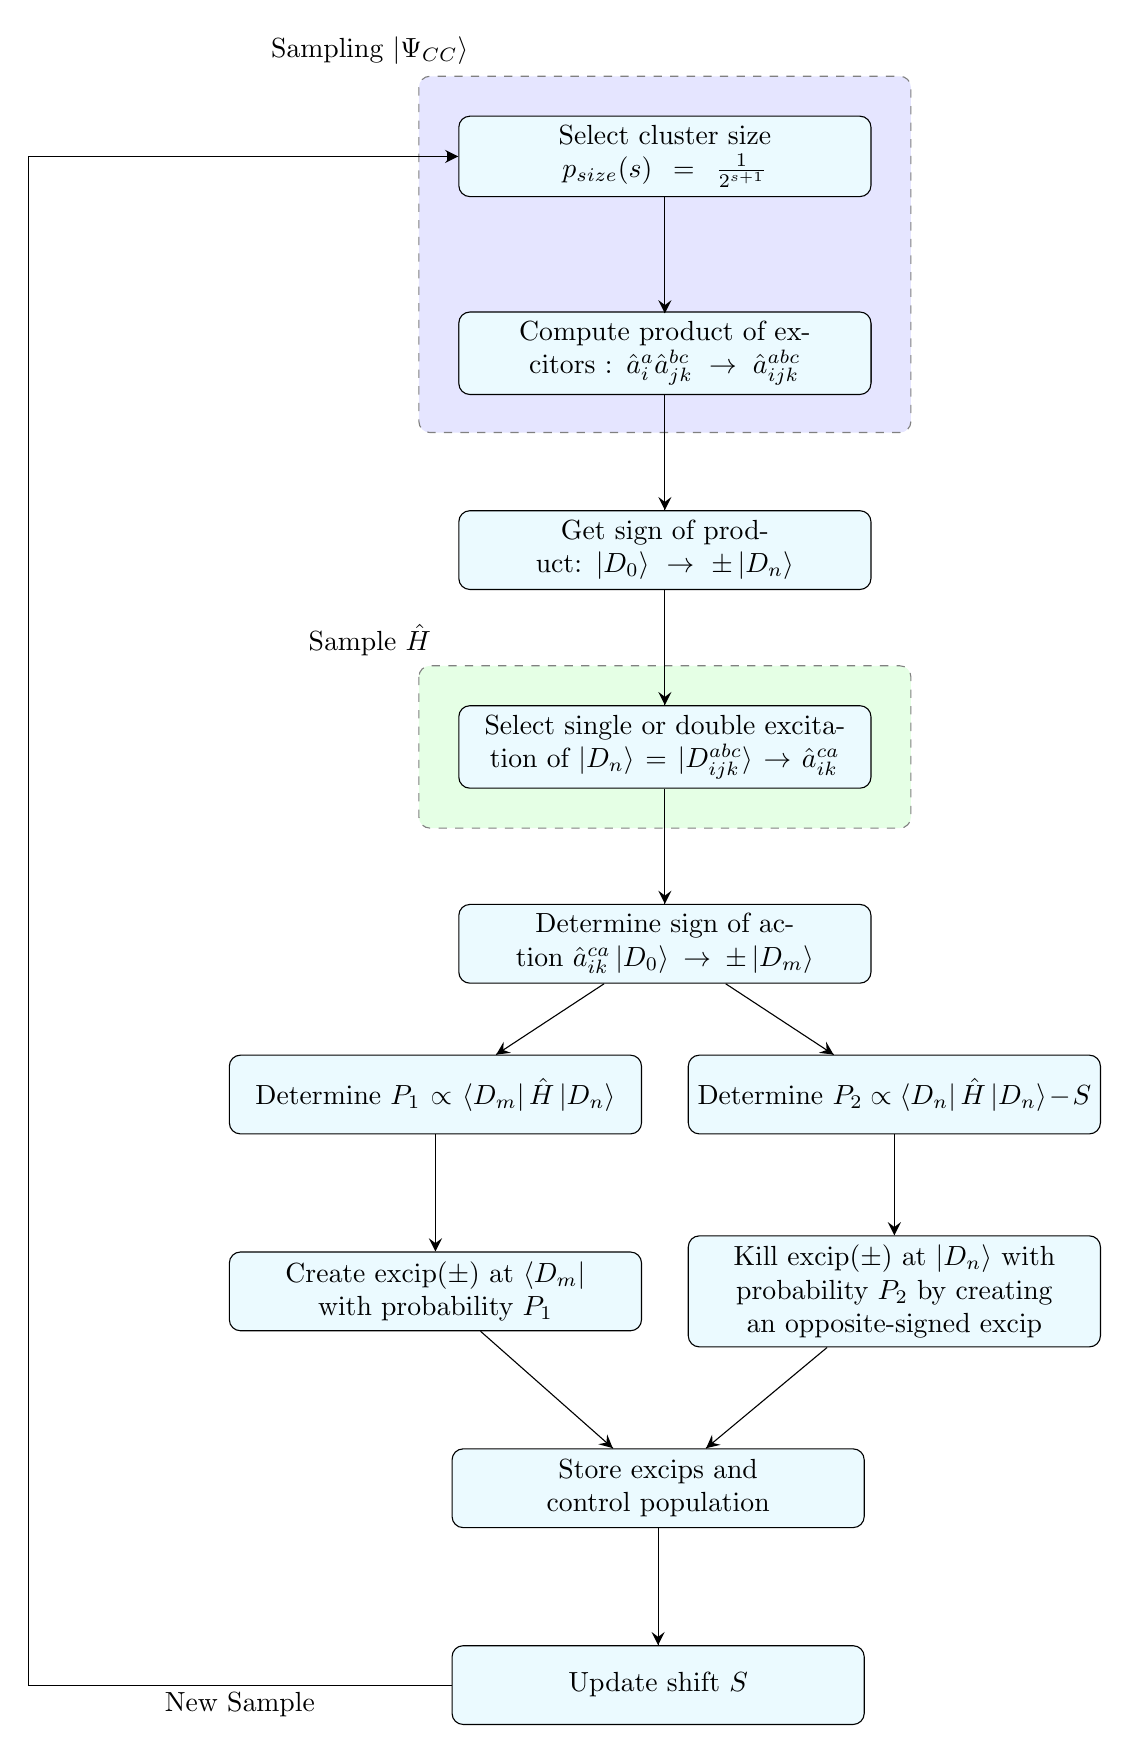
\begin{tikzpicture}[node distance=2cm]
		\node(SelectCluster)[roundrect]{Select cluster size  $p_{size}(s)=\frac{1}{2^{s+1}}$};% of one particle in one dimension};
		\node(ConstructCluster)[roundrect, below of=SelectCluster, yshift=-0.5cm]{Select excitations according to rules from tab. \ref{tab:cpluster}};
		\node(ProductCluster)[roundrect, below of=SelectCluster, yshift=-0.5cm]{ Compute product of excitors : $\hat{a}_{i}^{a}\hat{a}_{jk}^{bc} \rightarrow \hat{a}_{ijk}^{abc}$};
		\node(KetSign)[roundrect, below of=ProductCluster, yshift=-0.5cm]{Get sign of product: $\ket{D_0} \rightarrow \pm \ket{D_n}$};
		\node(SelectBra)[roundrect, below of=KetSign, yshift=-0.5cm]{Select single or double excitation of $\ket{D_n} = \ket{D_{ijk}^{abc}} \rightarrow \hat{a}_{ik}^{ca}$};
		\node(BraSign)[roundrect, below of=SelectBra, yshift=-0.5cm]{Determine sign of action $\hat{a}_{ik}^{ca}\ket{D_0} \rightarrow \pm \ket{D_m} $ };
		\node(Offdiagonal)[roundrect, below left of=BraSign, yshift=-0.5cm, xshift=-1.5cm ]{Determine $P_1 \propto \bra{D_m}\hat{H} \ket{D_n}$};
		\node(Diagonal)[roundrect, below right of=BraSign, yshift=-0.5cm,xshift=1.5cm]{Determine $P_2 \propto \bra{D_n}\hat{H} \ket{D_n}-S$};
		\node(CreateExcip)[roundrect, below of=Offdiagonal, yshift=-0.5cm]{Create excip($\pm$) at $\bra{D_m}$ with probability $P_1$};
		\node(KillExcip)[roundrect, below of=Diagonal, yshift=-0.5cm]{Kill excip($\pm$) at $\ket{D_n}$ with probability $P_2$ by creating an opposite-signed excip};
		\node(StoreExcip)[roundrect, below of=KillExcip, yshift=-0.5cm, xshift=-3cm]{Store excips and control population};
		\node(TuneS)[roundrect, below of=StoreExcip, yshift=-0.5cm]{Update shift $S$ };
		\draw [arrow] (SelectCluster) -- (ConstructCluster);
		\draw [arrow] (ConstructCluster) -- (ProductCluster);
		\draw [arrow] (ProductCluster) -- (KetSign);
		\draw [arrow] (KetSign) -- (SelectBra);
		\draw [arrow] (SelectBra) -- (BraSign);	
		\draw [arrow] (BraSign) -- (Offdiagonal);
		\draw [arrow] (BraSign) -- (Diagonal);
		\draw [arrow] (Offdiagonal) -- (CreateExcip);
		\draw [arrow] (Diagonal) -- (KillExcip);
		\draw [arrow] (KillExcip) -- (StoreExcip);
		\draw [arrow] (CreateExcip) -- (StoreExcip);
		\draw [arrow] (StoreExcip) -- (TuneS);
		\draw [arrow,rectangle connector=-8cm] (TuneS) to node[descr] [anchor=north] {New Sample} (SelectCluster);
		%	\draw [arrow] (Check E) -- node [anchor=east]{Yes} (Finish);
		%\background{Setup system}{Set T2}{Calc CCDT}{Calc D10}{Wave-function}
		%\background{Setup system}{Set T2}{Calc CCDT}{Calc D10}{Wave-function}
		\begin{pgfonlayer}{background}
		% Compute a few helper coordinates
		\path (SelectCluster.west |- SelectCluster.north)+(-0.5,0.5) node (a) {};
		\path (ConstructCluster.south -| ConstructCluster.east)+(+0.5,-0.5) node (b) {};
		\path[fill=blue!10,rounded corners, draw=black!50, dashed]
		(a) rectangle (b);
		\path (a.west |- a.north)+(-0.5,0.2) node (atext) {Sampling $\ket{\Psi_{CC}}$};
		\end{pgfonlayer}
		\begin{pgfonlayer}{background}
		% Compute a few helper coordinates
		\path (SelectBra.west |- SelectBra.north)+(-0.5,0.5) node (a) {};
		\path (SelectBra.south -| SelectBra.east)+(+0.5,-0.5) node (b) {};
		\path[fill=green!10,rounded corners, draw=black!50, dashed]
		(a) rectangle (b);
		\path (a.west |- a.north)+(-0.5,0.2) node (atext) {Sample $\hat{H}$};
		\end{pgfonlayer}
		\end{tikzpicture}
	\end{center}
	\caption{Flow chart for CCQMC sampling. } \label{figccqmcWF}
\end{figure}




\chapter{Results and discussion} \label{sec:Results}

\section{The CCD results}
As we have already mentioned the HEG is a very convenient system to study various many-body methods. In particular we have found many other researches who have implemented the CCD approximation for such system. That allow us to test our solution against results obtained in many other works on the topic. In particular we have compared our results with some other students from our department, namely with Miller \cite{millerAntumMechanicalStudies}, Hansen \cite{hansenCoupledClusterStudies} and \cite{gustavbaardsenCoupledclusterTheoryInfinite2014}. Table $\ref{tab:CCDcompar}$ present the comparison of the results. As one can see we manage to reproduce their results up to a chosen \textbf{tolerance} for CCD (in this case $10^{-6}$). 


\begin{landscape}
	\begin{table}[h]
		\centering

		\begin{tabular}{rrllll}
			$r_s$ & States & $\Delta E_{CCD}^{Miller}$ &$\Delta E_{CCD}^{Hansen}$  &$\Delta E_{CCD}^{Baardsen}$ & $\Delta E_{CCD}$\\
			\hline
			\hline
			1.0 & 54 & -0.3178228436889338 & -0.317822843688933   &           & -0.3178230699319593  \\
			1.0 & 66 & -0.3926965898061968 & -0.3926965898061966  &           & -0.3926968074770886  \\
			1.0 & 114 & -0.4479105961757175 & -0.4479105961757175 & -0.447909 & -0.4479109389185165  \\
			1.0 & 162 & -0.4805572589306421 & -0.4805572589306416 &           & -0.4805570782443642  \\
			1.0 & 186 & -0.4855229317521320 & -0.4855229317521318 & -0.485523 & -0.4855227418241649  \\
			1.0 & 246 & -0.4929245740023971 & -0.4929245740023975 &           & -0.4929243692209991  \\
			1.0 & 294 & -0.4984909094066806 & -0.4984909094066818 &           & -0.4984906939593084  \\
			1.0 & 342 & -0.5019526761547777 & -0.5019526761547779 &           & -0.5019524529049425  \\
			1.0 & 358 & -0.5025196736076414 & -0.502519673607641  & -0.502523 & -0.5025194488388953  \\ \hline
			0.5 & 114 & -0.5120153541478306 & -0.5120153541478306 & -0.512015 & -0.5120152296730573  \\
			0.5 & 186 & -0.5114620616957333 &                     & -0.553329 & -0.553329520936615   \\
			0.5 & 342 & -0.5729645498903680 & -0.572964549890367  &           & -0.572964399507112   \\
			0.5 & 358 & -0.5297417436322546 &                     & -0.573678 & -0.5736804143578936  \\ \hline    
			2.0 & 114 & -0.3577968843144996 & -0.3577968843144996 & -0.357798 & -0.3577955282575226  \\
			2.0 & 342 & -0.4014136184665558 & -0.4014136184665555 &           & -0.4014117905655014  \\
		\end{tabular}
				\captionsetup{width=1.1\textwidth}
				\caption{Our results for correlation energy in Hartree units for 14 electrons obtained by CCD solver $\Delta E_{CCD}$, presented with results from Miller \cite{millerAntumMechanicalStudies}, results from Hansen \cite{hansenCoupledClusterStudies} and results from Baardsen \cite{gustavbaardsenCoupledclusterTheoryInfinite2014}. 
				} \label{tab:CCDcompar}
	\end{table}
\end{landscape}
Another test is to compare our results with those from solver presented in \cite{hjorth-jensenAdvancedCourseComputational2017}. Table $\ref{tab:unittest}$ present data for a small number of electrons ($N_e=2$) and relatively small number of states ($N_s$). As one can see from the table the results for the energy are almost the same (up to machine precision).
\begin{table}[h]
	\centering

	\begin{tabular}{rlll}
		n & $\Delta E_{CCD}$     &   $\Delta E_{CCD}^{test}$  \\ \hline
		0 & -0.01833394188507821 & -0.0183339418850782  \\
		1 & -0.01864313296809337 & -0.01864313296809333 \\
		2 & -0.01860449158525421 & -0.01860449158525414 \\
		3 & -0.01860932269795203 & -0.01860932269795206 \\
		4 & -0.01860871870720909 & -0.01860871870720907 \\
	\end{tabular}
		\captionsetup{width=1\textwidth}
		\caption{Our results for correlation energy $\Delta E_{CCD}$  for $N_e=2$, $r_s=1$ and $N_s=66$,   tested against results  $\Delta E_{CCD}^{test}$ from \cite{hjorth-jensenAdvancedCourseComputational2017} CCD solver for the HEG. Mixing parameter is equal one. All values are in Hartree units.}
	\label{tab:unittest}
\end{table}
\subsubsection{Complete basis set and Thermodynamical limit}
In thermodynamical limit the number of particles should approaches infinity. However this is not the case for a real-life computations. And even for the finite number of particles it is hard to perform computations for large numbers, because even best many-body methods usually rapidly scale with size. A solution here is to perform computations for some different number of particles and then use extrapolation technique in order to obtain the limit.\\
In complete basis set limit (CBS) the number of single-particle wave functions should approach infinity. However this is also cannot be achieved for real-life computations. Normally we have to limit our basis to a certain number of basis functions. On Fig. $\ref{fig:CBS}$ one can see how the extrapolation technique is applied to obtain get the correlation energy in the CBS limit for HEG. Here we have used a so-called single-point extrapolation presented by Shepherd et al. in \cite{shepherdInvestigationFullConfiguration2012}. We have obtained value $-0.5142$ for the correlation energy, while Shepherd got $-0.5325(4)$. The result for CCQMC obtained by Thom is $-0.5155(3)$ \cite{spencerDevelopmentsStochasticCoupled2016}.

\begin{figure}[ht!]
	\centering
	\includegraphics[width=0.8\linewidth]{CCDvsCCDT}
	\caption{The correlation energy plotted against different $r_s$ the  electron gas, for $N_e=14$ and 54 single-particle states. CCDT results were taken from \cite{hansenCoupledClusterStudies}}
	\label{fig:CCDvsCCDT}
\end{figure}

\begin{figure}[ht!]
	\centering
	\includegraphics[width=0.8\linewidth]{cbs}
	\caption{The CBS limit for the 3D electron gas obtained by extrapolation of a second degree polynomial in $N_{states}^{-1}$. Here Miller's \cite{millerAntumMechanicalStudies} results for higher number of states([406 - 2090] were used. $N_e=14$ and limit $N_{states} \rightarrow \infty$ is -0.514204  }
	\label{fig:CBS}
\end{figure}



\subsubsection{Results for quantum dot}
We do not obtain a lot of results for QD as soon as our main system was HEG. However CCD solver we have developed for the HEG can be also used to compute ground state properties for QD. The results for QD is present in tables $\ref{tab:resultsHF}$ and  $\ref{tab:resultsCCD}$ and have been tested against the results obtained by Lohne in his master thesis for CCSD \cite{lohneCOUPLEDCLUSTERSTUDIESQUANTUM}. For the Hartree-Fock we obtain exactly the same results within the given precision ($10^{-6}$). 
The exact energy in case of  2 electrons and oscillator potential $\omega=1$ has been obtained analytically by Taut \cite{tautTwoElectronsExternal1993a}. It is equal exactly 3 a.u. We do not obtain this value, however the correlation energy for CCD brings us closer to this result. Unfortunately our program for QD is rather slow and we just tested it for the very simple case of two electrons. In the next Chapter we will discuss how it can be improved in order to get a significant speed up.  

\begin{table}[h!]
	\begin{center}
		\begin{tabular}{|c c| c c| c c| c c|}
			%\cline{1-12}
			%         & \multicolumn{1}{c}{N=2} & \multicolumn{5}{c}{N=6}  \\
			%\cline{1-12}
			\hline
			\multirow{2}{*}{} & 
			\multicolumn{1}{c}{$\omega$=0.1} \vline& 
			\multicolumn{2}{c}{$\omega$=0.5} \vline&
			\multicolumn{2}{c}{$\omega$=1} \vline&
			\multicolumn{2}{c}{$\omega$=2} \vline\\
			\hline
			$R$  & $\Delta E_{corr}$ & $R$ & $\Delta E_{corr}$ & $R$  & $\Delta E_{corr}$ &$R$ &  $\Delta E_{corr}$  \\
			\hline
			$  3 $   & $-0.084668$  &$ 3 $  & $-0.117877$  &$  3 $   & $-0.123643$   &$ 3$  & $-0.125520$   \\
			$  4 $   & $-0.084892$  &$ 4 $  & $-0.125975$  &$  4 $   & $-0.137418$   &$ 4$  & $-0.144715$   \\
			$  5 $   & $-0.082373$  &$ 5 $  & $-0.129695$  &$  5 $   & $-0.143977$   &$ 5$  & $-0.153792$   \\
			$  6 $   & $-0.082521$  &$ 6 $  & $-0.131944$  &$  6 $   & $-0.147998$   &$ 6$  & $-0.159730$   \\
			$  7 $   & $-0.082579$  &$ 7 $  & $-0.133271$  &$  7 $   & $-0.150504$   &$ 7$  & $-0.163497$   \\
			$  8 $   & $-0.082654$  &$ 8 $  & $-0.134251$  &$  8 $   & $-0.152288$   &$ 8$  & $-0.166194$   \\
			$  9 $   & $-0.082708$  &$ 9 $  & $-0.134938$  &$  9 $   & $-0.153566$   &$ 9$  & $-0.168154$   \\
			$  10$   & $-0.082749$  &$ 10$  & $-0.135473$  &$  10$   & $-0.154552$   &$ 10$ & $-0.169664$   \\
			$  11$   & $-0.082782$  &$ 11$  & $-0.135886$  &$  11$   & $-0.155319$   &$ 11$ & $-0.170848$   \\
			$  12$   & $-0.082808$  &$ 12$  & $-0.136220$  &$  12$   & $-0.155939$   &$ 12$ & $-0.171805$   \\
			\hline                                                                                    
		\end{tabular}
		\caption{Coupled Cluster Doubles correlation energy for QD for two electrons and different values of $\omega$ in atomic units. }   \label{tab:resultsCCD}
	\end{center}	
\end{table}
\begin{table}[h!]
	\begin{center}
		\begin{tabular}{|c c| c c| c c| c c|}
			%\cline{1-12}
			%         & \multicolumn{1}{c}{N=2} & \multicolumn{5}{c}{N=6}  \\
			%\cline{1-12}
			\hline
			\multirow{2}{*}{} & 
			\multicolumn{1}{c}{N=2} \vline& 
			\multicolumn{2}{c}{N=6} \vline&
			\multicolumn{2}{c}{N=12} \vline&
			\multicolumn{2}{c}{N=20} \vline\\
			\hline
			$R$  & $E_{HF}$ & $R$ & $E_{HF}$ & $R$  & $E_{HF}$ &$R$ &  $E_{HF}$  \\
			\hline
			$  3 $   & $3.16269$  &$ 3 $  & $21.593198$  &$  3 $   & $73.765549$   &$ 3$  & $-          $   \\
			$  4 $   & $3.16269$  &$ 4 $  & $20.766919$  &$  4 $   & $70.673849$   &$ 4$  & $177.963297 $   \\
			$  5 $   & $3.16192$  &$ 5 $  & $20.748402$  &$  5 $   & $67.569930$   &$ 5$  & $168.792442 $   \\
			$  6 $   & $3.16192$  &$ 6 $  & $20.720257$  &$  6 $   & $67.296869$   &$ 6$  & $161.339721 $   \\
			$  7 $   & $3.16191$  &$ 7 $  & $20.720132$  &$  7 $   & $66.934745$   &$ 7$  & $159.958722 $   \\
			$  8 $   & $3.16191$  &$ 8 $  & $20.719248$  &$  8 $   & $66.923094$   &$ 8$  & $158.400172 $   \\
			$  9 $   & $3.161909$ &$ 9 $  & $20.719248$  &$  9 $   & $66.912244$   &$ 9$  & $158.226013 $   \\
			$  10$   & $3.161909$ &$ 10$  & $20.719217$  &$  10$   & $66.912035$   &$ 10$ & $158.226030 $   \\
			$  11$   & $3.161909$ &$ 11$  & $20.719216$  &$  11$   & $66.911365$   &$ 11$ & $158.010277 $   \\
			$  12$   & $3.161909$ &$ 12$  & $20.719216$  &$  12$   & $66.911364$   &$ 12$ & $158.004953 $   \\
			\hline                                                                                    
		\end{tabular}
		\caption{ Ground-state energies for QD measured in a.u. obtained numerically by Hartree-Fock method for different number of shells (R) and electrons (N).  Oscillator strength $\omega=1$.}   \label{tab:resultsHF}
	\end{center}
\end{table}


\section{The CCQMC results}
CCQMC is a population dynamics algorithm. That require for it to reproduce a certain behavior for the population of walkers, or in our case excips. That means that the validity of our CCQMC results is based on getting the proper population dynamics for the excips. On the other hand for this particular algorithm the sing structure of excips should be correct. \\
For the HEG we do not have single excitations and have to deal only with doubles. When we perform the computation for the deterministic CCD this was a huge advantage. However, it might not be so for the CCQMC, because it impose limits on our ability to spawn excips in the system. \\
Let's consider how this is done for our simulation. We only have three different cluster sizes in our simulation: cluster size one, two and three. The cluster size one is the cluster with zero excitors and there is only one such cluster, which is reference determinant. As soon as we can spawn only double or single excitation from the selected cluster this leave us with only doubles being spawned from reference. In the beginning of simulation, before we start population control, the death also prohibited for the reference, so it's population never decrease at this point. For the cluster size one we are not able to spawn any excips, because we do not consider quadruples and do not have singles at the same time, so the only possibility here is death for the excips spawned before. After we start population control the probability for excips to die changes, but it still no other outcomes possible on this step. For the cluster size three both spawning and death could be possible is we include quadruples. However we do not have them from previous steps, so death on this step never occurs and the only possible outcome here is to spawn a doubly excited excip. This happens due to the only existing excitors are doubles and that means we can only create a composite cluster combining two doubles and getting a quadrupole excitation. The absence of singles leave us with much less possibilities to spawn and/or kill excips and this introduce some difficulties in analyzing the population dynamics of the simulation.\\
In order to obtain a valid results from the simulation one first have to reach a so-called "plateau". As it have been presented in the article by Thom and Spencer \cite{spencerDevelopmentsStochasticCoupled2016} one can adjust simulation parameters in a way that plateau become easy to spot on a plot. Fig. $\ref{fig:thomEG}$ present the results they have obtained for the neon atom for CCQDSTQ approximation. Despite the fact that we do not take into account higher excitation it could be a valid test if we could reproduce the same behavior in our simulation. The obvious difficulty here is the fact that we have to be vary careful choosing the parameters for the simulation and the fact that we are very limited in our ability to tune them all at the same time. One of the solutions here might be to fix some of them for a while and investigate the behavior of the system. We decide to fix population on reference determinant and run the simulation. The population dynamics should be close to those obtained by Thom and Spencer. Fig. $\ref{fig:nx2k}$ present the population dynamics we got for 14 electrons and 54 states. As one can see from the plot the plateau is reached for the critical number of excips being between $10^3$ and $10^4$, which is a result we expected to get for the $r_s=0.5$. This value was chosen because as one can see from Fig.On Fig. $\ref{fig:CCDvsCCDT}$ the difference between CCSD and CCSDT for electron gas decreases for smaller $r_s$. We also run the simulation for 162 basis functions and observe a growth in number of excips - it become closer to $10^4$. From such population dynamics one may assume that we got a proper sign structure. However this results are obtained for fixed normalization and it might introduce some bias in the simulation. 





\begin{figure}[ht!]
	\centering
	\includegraphics[width=0.8\linewidth]{thomEG}
	\caption{Ne cc-pVQZ CCSDTQ calculations starting with different initial
		particle numbers at the reference and different timesteps. (a): With a carefully
		chosen low timestep and initial population, a plateau is visible. An increased
		timestep and initial population overshoot the plateau but have a shoulder.
		The lower panel shows a maximum of the particle ratio at the position of
		the shoulder and plateau. (b): "Shoulder plots" allow shoulder height to be
		read off easily and calculations compared. Reproduced from \cite{spencerDevelopmentsStochasticCoupled2016}, with the permission of AIP Publishing. }
	\label{fig:thomEG}
\end{figure}


\begin{figure}[ht!]
	\centering
	\includegraphics[width=0.8\linewidth]{Nex2000new}
	\caption{The population dynamics of excips for $N_e=14$, 54 basis functions. $r_s=0.5$, $\delta \tau=0.0005$.}
	\label{fig:nx2k}
\end{figure}




\begin{figure}[ht!]
	\centering
	\includegraphics[width=0.8\linewidth]{Nex20000}
	\caption{The population dynamics of excips for $N_e=14$, 54 basis functions, $r_s=0.5$, $\delta \tau=0.0005$ with the population control. enabled after $5\cdot 10^3$ iterations. Damping parameter  $\gamma = 0.05$ and $A=5$.}
	\label{fig:nx20k}
\end{figure}


\begin{landscape}
	\begin{figure}[ht!]
		\centering
		\includegraphics[width=0.8\linewidth]{platFind}
		\caption{Population dynamics, $N_e=14$, $r_s=0.5$, no population control.}
		\label{fig:platFind}
	\end{figure}
\end{landscape}

\begin{landscape}
	\begin{figure}[ht!]
		\centering
		\includegraphics[width=0.8\linewidth]{platFindStune}
		\caption{Population dynamics, $N_e=14$, $r_s=0.5$, $\delta \tau=0.0001$, 54 basis functions  with population control. Damping parameter $\gamma = 0.05$. }
		\label{fig:platFindStune}
	\end{figure}
	
\end{landscape}



\clearpage

\part{Conclusion further research}
\chapter{Conclusion}

In this thesis we have studied many-body problems for the electron gas and quantum dots. Various methods have been used:  Hartree-Fock,  coupled cluster for doubles and also very recently presented in literature stochastic coupled cluster method. 


\chapter{Further research}
In this master thesis we have implemented deterministic CCD method for HEG and QD. The results from these two agree with what have been done so far by other researchers. It is possible to improve our solvers implementing so-called intermediates for the amplitudes. This technique is described in \cite{hjorth-jensenAdvancedCourseComputational2017}.  For the QD it is possible to use smart storage of matrix elements as it has been done here \cite{leikangerFullConfigurationInteraction}. Moreover the CCSD algorithm can be implemented based on already developed code for CCD. \\
The CCQMC solver is now available only for the HEG, so it is natural to extend it to the QD as well. This might be even a better option as soon as for QD we are able to create single excitations and the population dynamics can be much better and easier to analyse.\\
It is also a possibility to extend the CCQMC for Triples and Quadruples. However before doing some improvements should be done to speed up the program. The very straightforward improvement is to apply parallelization of the code using MPI. \\
In this thesis we only focus on unlinked coupled cluster equations, however there it is possible to perform simulation for linked coupled cluster Monte Carlo, as it has been done here \cite{franklinLinkedCoupledCluster2016}.



\clearpage
\newpage
**\appendix
\chapter{Matrix Elements of Hamiltonian}\label{app:1}
It is convenient to introduce formulas for different matrix elements of Hamiltonian. \\
Matrix elements between determinants that differs more then two orthonormal spin orbitals are zero by construction, so we are not going to consider such term.\\
Let us choose one determinant to be single or double excitation on another. \\
For double excitation:
\begin{equation}
\ket{\Phi_{m}}=a^\dagger_r a^\dagger_s a_q a_p \ket{\Phi_n}.
\end{equation}
In this case the corresponding matrix element then is:
\begin{equation}
\bra{\Phi_n} \hat{H}\ket{\Phi_{m}}=\braket{rs|pq}_{AS}.
\end{equation}
For single excitation:
\begin{equation}
\ket{\Phi_{m}}=a^\dagger_r  a_p \ket{\Phi_n}.
\end{equation}
And corresponding matrix element then is:
\begin{equation}
\bra{\Phi_n} \hat{H}\ket{\Phi_{m}}=\sum_{k}^{N-1}\braket{rk|pk}_{AS}.
\end{equation}
here sum runs over all common orbitals present in the determinants.\\
We also need to compute the diagonal matrix element:
\begin{equation}
\bra{\Phi_n} \hat{H}\ket{\Phi_{n}}=\sum_{p\in n} \braket{p|\hat{h}|p} + \frac{1}{2} \sum_{p,q \in n}^{N-1}\braket{pq|pq}_{AS}.
\end{equation}

\chapter{Coulomb matrix elements}\label{app:2}
In the article by Anisimovas and Matulis \cite{anisimovasEnergySpectraFewelectron1998} there is an algorithm to compute a Coulomb matrix elements in a closed form. The final expression is the following:


\begin{align}
& \braket{12|V|34}= \delta_{m_1+m_2,m_3+m_4} \;  \left[ \prod_{i=1}^4 \frac{n_i !}{(n_i+|m_i|!)} \right]^{1/2}  \nonumber \\
&\times \sum_{(4)j=0}^{n} \Bigg[ \frac{(-1)^{j_1+j_2+j_3+j_4}} {j_1!j_2!j_3!j_4!} \; \left[ \prod_{k=1}^4 \begin{pmatrix} n_k+|m_k|\\n_k-j_k\end{pmatrix}  \right]  \; \frac{1}{2^{\frac{G+1}{2}}} \nonumber  \\
&\times \sum_{(4)l=0}^{\gamma}\left( \delta_{l_1,l_2} \; \delta_{l_3,l_4} \; (-1)^{\gamma_2+\gamma_3-l_2-l_3} \left[ \prod_{t=1}^4 \begin{pmatrix} \gamma_t\\l_t\end{pmatrix} \right] \; \Gamma \left(1+\frac{\Lambda}{2} \right) \; \Gamma \left(\frac{G - \Lambda +1}{2}\right)    \right)  \Bigg]
\end{align} 
here
\begin{align*}
&\gamma_1=j_1+j_4+\frac{|m_1|+m_1}{2}+\frac{|m_4|-m_4}{2} \\
&\gamma_2=j_2+j_3+\frac{|m_2|+m_2}{2}+\frac{|m_3|-m_3}{2} \\
&\gamma_3=j_3+j_2+\frac{|m_3|+m_3}{2}+\frac{|m_2|-m_2}{2} \\
&\gamma_4=j_4+j_1+\frac{|m_4|+m_4}{2}+\frac{|m_1|-m_1}{2} \\
&G=\sum_{i}^4 \gamma_i, \text{   }  \Lambda = \sum_{i}^4 l_i, \text{   } \sum_{(4)j=0}^{n}=\sum_{j_1=0}^{n_1}\sum_{j_2=0}^{n_2}\sum_{j_3=0}^{n_3}\sum_{j_4=0}^{n_4}\\
\end{align*}
This matrix elements are computed using function \textit{Coulomb$\_$HO} realized in class \textit{Coulomb$\_$Functions}. One should be careful because it does not include spin.



\chapter{Some additional calculations on sampling probabilities}\label{app:3}

Number of single-, double- and triple-excitations including Pauli exclusion principle are defined by the following formulas:

\begin{equation}\label{eq:num_singles}
N_s = \frac{1}{2}F(N-F)
\end{equation}

\begin{equation}\label{eq:num_doubles}
N_d = \frac{1}{2^4}F(F-2)(N-F)^2
\end{equation}

\begin{equation}\label{eq:num_triples}
N_t = \frac{1}{2^4}F(3F-4)(N-F)^3
\end{equation}
Where $F$ is the Fermi level and $N$ is the number of single-particle states in the system. So we choose single or double proportionally to their amount for a given system configuration.
\begin{equation}
P_1 = \frac{A \delta \tau \bra{D_m}\hat{H} \ket{D_n}}{p_{\text{select}}p_{sel}p_{\text{clust}}p_{\text{excit}}}
\end{equation}
\begin{equation}
P_2 = \frac{A \delta \tau (\bra{D_n}\hat{H} \ket{D_n}-S)}{p_{\text{select}}p_{sel}p_{\text{clust}}}
\end{equation}
where
\begin{equation}
\delta \tau \leq \frac{2}{E_{max} - S}
\end{equation}
where $E_{max}$ is the largest eigenvalue of the most excited determinant available in a given one-electron basis and $S \approx E_0$.\\
Parameter A is known as amplitude total amplitude of the cluster. It depends on size of the cluster.
\begin{equation}
A = N_0  \prod_{i=1}^s \frac{N_i}{N_0}
\end{equation},
where $N_i$ -- is population on the excip number $i$.

We select cluster size according exponential distribution:
\begin{equation}
p_{size}(s)=\frac{1}{2^{s+1}}
\end{equation}

\begin{equation}
p_{\text{clust}} (e|s)= s! \prod_{i=1}^s \frac{|N_i|}{N_{ex}}.
\end{equation}
Represents number of possibilities to choose excitations (excitors) within chosen cluster. Also $N_{ex}$ is total number of excited determinants that can by sampled in the system (doubles, if we choose CCD method). This number can be calculated using equations ($\ref{eq:num_singles}$),($\ref{eq:num_doubles}$) and ($\ref{eq:num_triples}$).

\begin{equation}
p_{select}(e)= p_{size}(s) p_{\text{clust}} (e|s) =  \frac{s!\prod_{i=1}^{s} |N_i|}{2^{s+1}N_{ex}}.
\end{equation}



\begin{equation}
p_{sel}= 1+N_{s}+N_{d}+N_{t}.
\end{equation}
$p_{sel}$ represent a number of samples in each time-step. This parameter must by constant and depend on total number of possible excited determinants combine with reference.


\begin{equation}
p_{\text{excit}} = \frac{1}{N_{ex}}.
\end{equation}
This parameter represent probability to select excited state (not reference).


Lets compute some particular probabilities:\\



\begin{enumerate}
	\item For a cluster of size zero:
	
	\begin{align}
	p_{size} = \frac{1}{2},\\
	p_{sel} = 1+N_{s}+N_{d}+N_{t} = 2N_0,\\
	p_{excit}=\frac{1}{N_{ex}} = \frac{1}{N_d}, for doubles\\
	A = N_0,\\
	p_{clust}=1\\
	\delta \tau = \frac{2}{E_m  - S},\\
	p_{death}=0, by constraction\\
	p_{spawn} = \frac{2}{|E_m  - S|} \frac{|AH_{m0}|}{ p_{sel}  p_{size} p_{clust}p_{excit} }=
	\frac{2}{|E_m  - S|} \frac{N_0|H_{m0}|}{ \frac{1}{2}  2N_0 \frac{1}{N_d} }=\\
	p_{spawn} = \frac{2N_d|H_{m0}|}{|E_m  - S|} 
	\end{align}
	
	\item For cluster size 1 we have three possibilities:\\
	1) Parent is a singly exited determinant.
	
	\begin{itemize}
		\item no spawn
		\item death according to:
		\begin{align}
		p_{size} = \frac{1}{4},\\
		p_{sel} =  2N_0,\\
		p_{excit}= \frac{1}{N_d}\\
		A = N_0\frac{N_i}{N_0}=N_i,\\
		p_{clust}=1!\frac{1}{N_0}\\
		\delta \tau = \frac{2}{E_m  - S},\\
		p_{death} = \frac{2}{|E_m - S|} \frac{|A(H_{mm}-S)|}{ p_{sel}  p_{size} p_{clust} }=\\
		\frac{4}{|E_m  - S|} \frac{|H_{mm}-S|N_dN_i}{N_0 }
		\end{align}
		here $N_i$ population on chosen excip $i$. Normally in the beginning of simulation it is $i= +1,-1$.
	\end{itemize}
	
	2) Parent is a doubly exited determinant.
	
	\begin{itemize}
		\item can spawn only singly excited determinant with probability:
		\begin{align}\label{eq:spawn_ziae_1}
		p_{spawn} = \frac{2}{E_m - S} \frac{|AH_{mn}|}{ p_{sel}  p_{size} p_{clust} p_{excit} }=\\
		\frac{2}{|E_m  - S|} \frac{|H_{mn}|}{2N_0 \frac{1}{4} \frac{1}{N_d} \frac{1}{N_0}} =\\
		p_{spawn} =\frac{4|H_{mn}|N_d}{|E_m  - S|}
		\end{align}
		\item death according to:
		\begin{align}
		p_{death} = \frac{2}{E_m - S} \frac{|A(H_{mm}-S)|}{ p_{sel}  p_{size} p_{clust} }= \frac{2}{|E_m - S|} \frac{A|H_{mm}-S|N_i}{ 2N_0 \frac{1}{4} \frac{1}{N_0}}=\\
		p_{death} = \frac{4|H_{mm}-S|N_i}{|E_m - S|} 
		\end{align}
	\end{itemize}
	3) Parent is a triply exited determinant.
	\begin{itemize}
		\item can spawn only singly or doubly excited determinant with same probability as before ($\ref{eq:spawn_ziae_1}$).
		\item $p_{death} = 1$ as we do not count triples.
	\end{itemize}
	
	\item For cluster size 2 we have two possibilities:\\
	1) Parent is a doubly exited determinant.
	\begin{itemize}
		\item can spawn only singly excited determinant with probability:
		\begin{align}
		p_{size} = \frac{1}{8},\\
		A = N_0\frac{N_i}{N_0}\frac{N_j}{N_0}=\frac{N_jN_i}{N_0},\\
		p_{clust}=2!\frac{|N_i|}{N_0}\frac{|N_j|}{N_0}=\frac{2|N_jN_i|}{N_0^2}\\
		\delta \tau = \frac{2}{E_m  - S},\\
		p_{spawn} = \frac{2}{|E_m - S|} \frac{|A(H_{mn}-S)|}{ p_{sel}  p_{size} p_{clust} p_{excit}  }=\\
		p_{spawn} = \frac{2}{|E_m - S|} \frac{  | \frac{N_jN_i}{N_0} (H_{mn}-S)|}{2N_0 \frac{1}{8} \frac{2|N_jN_i|}{N_0^2} \frac{1}{N_d} }=\\
		p_{spawn} = \frac{4}{|E_m - S|} \frac{ |\frac{N_jN_i}{N_0} (H_{mn}-S)|}{ \frac{|N_jN_i|}{N_0} \frac{1}{N_d} }=\frac{4|H_{mn}-S|N_d}{|E_m - S|}\label{eq:spawn_ziae_2}
		\end{align}
		\item death according to:
		\begin{align}
		p_{death} = \frac{2}{E_m - S} \frac{A|H_{mm}-S|}{ p_{sel}  p_{size} p_{clust} }=
		\frac{2}{E_m - S} \frac{\frac{N_jN_i}{N_0}|H_{mm}-S|}{ 2N_0 \frac{1}{8} \frac{2N_jN_i}{N_0^2} }=\\
		p_{death} =  \frac{4|H_{mn}-S|}{|E_m - S|}
		\end{align}
	\end{itemize}
	3) Parent is a triply exited determinant.
	\begin{itemize}
		\item can spawn only singly or doubly excited determinant with same probability as before ($\ref{eq:spawn_ziae_2}$).
		\item $p_{death} = 1$ as we do not count triples.
	\end{itemize}
	
	\item Cluster size 3:
	
	Parent is a triply exited determinant.
	\begin{itemize}
		\item can spawn only singly or doubly excited determinant with  probability  
		\begin{align}
		p_{size} = \frac{1}{16},\\
		A = N_0\frac{N_i}{N_0}\frac{N_j}{N_0}\frac{N_k}{N_0}=\frac{N_jN_iN_k}{N_0^2},\\
		p_{clust}=3!\frac{|N_i|}{N_0}\frac{|N_j|}{N_0}\frac{|N_k|}{N_0}=\frac{6|N_jN_iN_k|}{N_0^3}\\
		\delta \tau = \frac{2}{E_m  - S},\\
		p_{spawn} = \frac{2}{E_m - S} \frac{|A(H_{mn}-S)|}{ p_{sel}  p_{size} p_{clust} p_{excit}  }=\\
		p_{spawn} = \frac{2}{E_m - S} \frac{\frac{|N_jN_iN_k|}{N_0^2}|H_{mn}-S|}{ 2N_0 \frac{1}{16} \frac{6|N_jN_iN_k|}{N_0^3} \frac{1}{N_d}}= \\
		p_{spawn} = \frac{8N_d|H_{mn}-S|}{3(E_m - S)}
		\end{align}
		\item $p_{death} = 1$ as we do not count triples.
	\end{itemize}
\end{enumerate}



\printbibliography 



\end{document}